\chapter{Modeling laser atom interactions}
\label{cha:numberic_methods}
In order to study laser atom interactions on the attosecond time scale, one must developed or implemented a variety of numerical and analytic tools. Sec.~\ref{sec:TDSE} introduce the Time-dependent Schr\"odinger equation (TDSE), Sec.~\ref{sec:perturbation_theory} introduces the perturbative solution to the TDSE, Sec.~\ref{sec:numerical_methods} gives the details for how we solve the TDSE numerically, Sec.~\ref{sec:SAE} discusses the various single active electron (SAE) potentials used to model atoms other than Hydrogen, Sec.~\ref{sec:laser_pulses} provides details on the laser pulses utilized in the calculations including a frequency correction we helped develop, and Sec.~\ref{sec:observables} provides details on how the various observables are calculated.

%%%%%%%%%%%%%%%%%%%%%%%%%%%%%%%%%%%%%%%%%%%%%%%%%%%%%%%%%%%%%%%%%%%%%%%%%%%%%%%%%%%%%%%%%%%%%%%%%%%%%%%%%%%%%%%%%%
%%%%%%%%%%%%%%%%%%%%%%%%%%%%%%%%%%%%%%%%%%%%%%%%%%%%%%%%%%%%%%%%%%%%%%%%%%%%%%%%%%%%%%%%%%%%%%%%%%%%%%%%%%%%%%%%%%
%%%%%%%%%%%%%%%%%%%%%%%%%%%%%%%%%%%%%%%%%%%%%%%%%%%%%%%%%%%%%%%%%%%%%%%%%%%%%%%%%%%%%%%%%%%%%%%%%%%%%%%%%%%%%%%%%%
%%%%%%%%%%%%%%%%%%%%%%%%%%%%%%%%%%%%%%%%%%%%%%%%%%%%%%%%%%%%%%%%%%%%%%%%%%%%%%%%%%%%%%%%%%%%%%%%%%%%%%%%%%%%%%%%%%
%%%%%%%%%%%%%%%%%%%%%%%%%%%%%%%%%%%%%%%%%%%%%%%%%%%%%%%%%%%%%%%%%%%%%%%%%%%%%%%%%%%%%%%%%%%%%%%%%%%%%%%%%%%%%%%%%%
\section{Time-dependent Schr\"odinger equation}
\label{sec:TDSE}
The TDSE can be written as
\begin{equation}
    i\frac{\partial}{\partial t}\psi(\mathbf{r},t) = \hat{H}\psi(\mathbf{r},t)
    \label{eq:TDSE}
\end{equation}
where $i=\sqrt{-1}$ is the imaginary number, $\hat{H}$ is the Hamiltonian which describes the system, and $\psi(\mathbf{r},t)$ is the time dependent wavefunction. The Hamiltonian for a system with $N_e$ correlated electrons interacting with a laser field and $N_n$ fixed nuclei is
\begin{equation}
    \label{eq:atoms_and_molecules}
    \hat{H} = \sum_{e=1}^{N_e}\left(\frac{\hat{\mathbf{p}}^2_e}{2} + V_{las}(\mathbf{r},t) - \sum_{n=1}^{N_n} \frac{Z_n}{r_{e,n}}\right) + \sum_{e_1 < e_2=1}^{N_e}\frac{1}{r_{e_1, e_2}}
\end{equation}
where $\hat{\mathbf{p}_e}=(-i\nabla_e)$ is the momentum operator of the $e^{th}$ electron, $V_{las}(\mathbf{r},t)$ is the laser operator, $Z_n$ is the charge of the $n^{th}$ nucleus, and $r_{i,j}$ is the Euclidean distance between particles $i$ and $j$. The laser interaction is typically considered using both the dipole and non-relativistic approximation in either the length gauge ($V_{las} = - \mathbf{E}(t)\cdot \mathbf{x}$) or velocity gauge ($V_{las} = - \mathbf{A}(t)\cdot \hat{\mathbf{p}}_e / c$). No analytic solution for more than one electron in a central potential are know as the problem is not separable. Therefore numerical methods are required. Solving the TDSE accurately in full dimensions for more than one electron is extremely difficult and next to impossible for three or more active electrons. For most studies, we make the single active electron approximation (SAE) where all except one 'active' electron and the nuclei are fixed in space. A SAE potential generated by the nuclei and remaining electrons is then used to model the interaction of the active electron with the fixed electrons and nuclei. The SAE Hamiltonian of an atom interacting with a laser field therefore becomes 
\begin{equation}
    \label{eq:SAE}
    \hat{H} = \frac{\hat{\mathbf{p}}^2}{2} + V_{las}(\mathbf{r},t) + V_{SAE}(r),
\end{equation}
where $V_{SAE}(r)$ is the SAE potential. The exact form of the SAE potentials used in this work is given in Sec.~\ref{sec:SAE}. Extensions on two-active electron calculation beyond the SAE approximation are discussed in Chapter~\ref{cha:electron_correlation}. Finally, it is often convenient to split the problem into a field free Hamiltonian ($\hat{H}_0$) and the time dependent laser field such that 
\begin{equation}
    \label{eq:field_free}
    \hat{H} = \hat{H}_0 + V_{las}(\mathbf{r},t).
\end{equation}
The resulting $H_0$ is time independent and its associated Eigenfunctions can be use to analyze the results of a simulation. 


%%%%%%%%%%%%%%%%%%%%%%%%%%%%%%%%%%%%%%%%%%%%%%%%%%%%%%%%%%%%%%%%%%%%%%%%%%%%%%%%%%%%%%%%%%%%%%%%%%%%%%%%%%%%%%%%%%
%%%%%%%%%%%%%%%%%%%%%%%%%%%%%%%%%%%%%%%%%%%%%%%%%%%%%%%%%%%%%%%%%%%%%%%%%%%%%%%%%%%%%%%%%%%%%%%%%%%%%%%%%%%%%%%%%%
%%%%%%%%%%%%%%%%%%%%%%%%%%%%%%%%%%%%%%%%%%%%%%%%%%%%%%%%%%%%%%%%%%%%%%%%%%%%%%%%%%%%%%%%%%%%%%%%%%%%%%%%%%%%%%%%%%
%%%%%%%%%%%%%%%%%%%%%%%%%%%%%%%%%%%%%%%%%%%%%%%%%%%%%%%%%%%%%%%%%%%%%%%%%%%%%%%%%%%%%%%%%%%%%%%%%%%%%%%%%%%%%%%%%%
%%%%%%%%%%%%%%%%%%%%%%%%%%%%%%%%%%%%%%%%%%%%%%%%%%%%%%%%%%%%%%%%%%%%%%%%%%%%%%%%%%%%%%%%%%%%%%%%%%%%%%%%%%%%%%%%%%
\section{Perturbation theory} % (fold)
\label{sec:perturbation_theory}
In the case of a weak laser field (typically intensities $<10^{13}$ W/cm$^2$) relative to the atomic potential the TDSE can be solved using perturbation theory (PT). In some cases, such as for the hydrogen atom, the corresponding terms of the perturbation series can be solved analytically. However, for many of the SAE potentials that we use there is no analytic solutions. In such a case, a numerical solution to the first-order terms of the series provides much of the same insight. 

Therefore, it is advantageous to provide a general framework that can be used for both analytical and numerical solutions. We start by diagonalizing the field free Hamiltonian $H_0$ to discretize both the bound (Sec.~\ref{sub:bound_state_calculations}) and continuum states (Sec.~\ref{sub:continuum_states}). The result can be written as a Green's function 
\begin{equation}
\label{eq:pt_green_func}
    G_0(t,t') = \SumInt_g e^{-iE_g t}\ket{\phi_g(t)}\bra{\phi_g(t')} e^{iE_g t'},
\end{equation}
where $\ket{\phi_g(t)}$ are the field free states (both bound and continuum), $E_g$ is the energy of the state, and $t$ denotes time. For some initial wavefunction $\ket{\Psi_0(\mathbf{r},t)}$, the consecutive orders of the PT can be obtained via
\begin{equation}
    \ket{\Psi_{i+1}(\mathbf{r},t)} = \int_{-\infty}^t dt_1 G_0(t,t_1)V_{las}(t_1)\ket{\Psi_i(\mathbf{r},t_1)}, 
\end{equation}
with $i = 0, 1, 2, \ldots$.
The total wavefunction in $N$th order can then be obtained via a sum such that 
\begin{equation}
    \ket{\Psi(\mathbf{r},t)}^{(N)} = \sum_i^N \ket{\Psi_{i}(\mathbf{r},t)}.
\end{equation}
By taking $N \rightarrow \infty$, the resulting wavefunction is exact in the regime where the perturbation is small as compared to other interaction terms. However, if the perturbation is of similar order as compared to other terms in the Hamiltonian, the series will not converge to the correct answer leading to the breakdown of PT. The wavefunction obtained using PT can be used to extract observables (Sec.~\ref{sec:observables}) in the same way as for a (full) numerical solution of the TDSE. Additionally, for laser-matter interactions PT offers the option to analyze the wavefunction of a particular order to extract further information about how many photons are involved in a process. 

\subsection{Selection rules} % (fold)
\label{sub:selection_rules}
The wavefunction is often expanded in 3D spherical harmonics to take advantage of selection rules for interactions with an electric field. We proceed by considering the selection rules for length gauge ($V_{las}=-\mathbf{E}\cdot \mathbf{r}$). For simplicity, we consider a linearly polarized laser field along the $z$-axis, i.e.
\begin{equation}
    V_{las}=-E_z z.
\end{equation}
Noting that $z=r\cos(\theta)$ we obtain
\begin{align}
    V_{las}&=-E_zr\cos(\theta)\\
    &=-2E_zr\sqrt{\frac{\pi}{3}}Y_1^0(\theta,\phi),
\end{align}
where $Y_\ell^m(\theta,\phi)$ is a spherical harmonic. This expansion can then be used to calculate the angular portion of a matrix element between two wavefunctions with $V_{las}$ as a perturbation: 
\begin{equation}
    \bra{Y_{\ell'}^{m'}}V_{las}\ket{Y_{\ell}^{m}} = -2E_zr\sqrt{\frac{\pi}{3}}\bra{Y_{\ell'}^{m'}}Y_1^0\ket{Y_{\ell}^{m}}.
\end{equation}
The integral over three spherical harmonics can be written as 
\begin{equation}
    \int_{4\pi} Y_{\ell_1}^{m_1*}Y_{\ell_2}^{m_2*}Y_{L}^{M} = \sqrt{\frac{(2\ell_1+1)(2\ell_2+1)}{4\pi(2L+1)}}\bra{\ell_1,0,\ell_2,0}\ket{L,0}\bra{\ell_1,m_1,\ell_2,m_2}\ket{L,M},
\end{equation}
where $\bra{\ell_1,m_1,\ell_2,m_2}\ket{L,M}$ is a Clebsch–Gordan coefficient. Thus, we get
\begin{align}
    \bra{Y_{\ell'}^{m'}}V_{las}\ket{Y_{\ell}^{m}} &= -E_zr\sqrt{\frac{(2\ell_1+1)(2\ell_2+1)}{3(2L+1)}}\bra{\ell',0,1,0}\ket{\ell,0}\bra{\ell',m',1,0}\ket{\ell,m},
\end{align}
which is only non-zero for $\ell' = \ell \pm 1$ and $m'=m$. Therefore, the selection rules for a linearly polarized laser along the $z$-axis are given by $\Delta\ell=\pm1$ and $\Delta m = 0$. Similarly, for a linearly polarized laser along either the $\hat{x}$ or $\hat{y}$ axis one gets $\Delta\ell=\pm1$ and $\Delta m = \pm1$. Finally, a circularly polarized laser in the $xy$-plane leads to $\Delta\ell=\pm1$ and $\Delta m = 1$ for absorbing a photon from a right-handed circularly polarized field and $\Delta\ell=\pm1$ and $\Delta m = -1$ for absorption of a photon from a left-handed circular polarized laser field. By taking advantage of these selection rules, one can greatly reduce the size of a wavefunction used in a particular order of PT or in a numerical TDSE solution.
% subsection selection_rules (end)

% section perturbation_theory (end)

%%%%%%%%%%%%%%%%%%%%%%%%%%%%%%%%%%%%%%%%%%%%%%%%%%%%%%%%%%%%%%%%%%%%%%%%%%%%%%%%%%%%%%%%%%%%%%%%%%%%%%%%%%%%%%%%%%
%%%%%%%%%%%%%%%%%%%%%%%%%%%%%%%%%%%%%%%%%%%%%%%%%%%%%%%%%%%%%%%%%%%%%%%%%%%%%%%%%%%%%%%%%%%%%%%%%%%%%%%%%%%%%%%%%%
%%%%%%%%%%%%%%%%%%%%%%%%%%%%%%%%%%%%%%%%%%%%%%%%%%%%%%%%%%%%%%%%%%%%%%%%%%%%%%%%%%%%%%%%%%%%%%%%%%%%%%%%%%%%%%%%%%
%%%%%%%%%%%%%%%%%%%%%%%%%%%%%%%%%%%%%%%%%%%%%%%%%%%%%%%%%%%%%%%%%%%%%%%%%%%%%%%%%%%%%%%%%%%%%%%%%%%%%%%%%%%%%%%%%%
%%%%%%%%%%%%%%%%%%%%%%%%%%%%%%%%%%%%%%%%%%%%%%%%%%%%%%%%%%%%%%%%%%%%%%%%%%%%%%%%%%%%%%%%%%%%%%%%%%%%%%%%%%%%%%%%%%
\section{Numerical Methods} % (fold)
\label{sec:numerical_methods}
For much of the parameter regime we are interested in, perturbation theory fails as an approximation method. Therefore, we have developed and implemented numerical solvers of the TDSE. As for most partial differential equations, numerical solutions to the TDSE have a relatively simple general form with the complexity hidden in the details. First, one chooses a basis/discretization to write down the solution, in our case the wavefunction. Next, the operators are expanded in the basis and written as a matrix. Then, one obtains a set of initial conditions at the start of the simulation, in our case typically a bound state of the atom or molecule. Finally, the initial condition is propagated in time with updates to the operating matrix between time steps. In this section, we will layout the basis/discretization choices in Sec.~\ref{sub:coordinate_systems}, followed by a detailed discussion of the implementation in the remaining subsections. For the sake of simplicity, we will focus on single active electron calculations in this section (for details on two-active electron calculation see Chapter~\ref{cha:electron_correlation}).



\subsection{Coordinate systems} % (fold)
\label{sub:coordinate_systems}
The solution to a single active electron calculation is three dimensional in space. The simplest and most general strategy would be to expand the wavefunction on a 3D grid in real space with the atom or molecule placed in the center. Such a grid is generated by discretizing each dimension (1D problem) with $N$ grid points and then taking a Kronecker product producing a 1D vector that represents the full 3D Cartesian space. The derivative operators can then be discretized utilizing finite differences (discussed in the next section) and stored in a matrix. The implementation is relatively straight forward and there are no assumptions about the symmetry of the problem. However, this method has its flaws. If a potential has a singularity, such as the Coulomb potential at zero ($V=-1/r$), special care must be taken to avoid sampling that point. Additionally, the size of the calculation scales like $N^3$ when the number of grid points in each dimension ($N$) increases. Therefore, obtaining converged results for large atoms, which require smaller grid spacing to sample the core properly, and high intensities, which require larger box sizes to keep the wavefunction on the grid, becomes computationally impractical. 
% for larger atoms and high intensity laser pulse, the number of points in each direction ($N$) increases. 
It is, therefore, useful to consider the symmetries of the problem in question to greatly speed up the calculations. Two standard approaches are to utilize cylindrical or spherical coordinates. 

The problem of an atom or a linear molecule aligned along a linearly polarized laser is cylindrically symmetric. Therefore, in this case the using cylindrical coordinates is the natural choice. By choosing the laser polarization (and internuclear axis) along the $z$-axis, the solution in the angular coordinate $\phi$ is given by the initial condition and can be given analytically. Thus, one only needs to find a solution in the $z$ and $\rho$ dimensions numerically, reducing the problem to two dimensions. As a result, solutions scale like $N^2$ which significantly accelerates calculations as compared to a 3D Cartesian code. 

However, in our studies we have actually found that spherical codes are often even faster. When written in spherical coordinates, the TDSE for a central potential (such as an atom) can be separated into a radial equation that contains the potential, and an angular portion that is independent of the potential. The angular solution can then be found analytically in the form of spherical harmonics and
the radial solution is all that remains. For the hydrogen atom an analytic solution exists. However, in general for a radial potential it is not guaranteed that there is an analytic solution. Therefore, we expand the wavefunction in spherical harmonics and use finite difference to discretize the radial portion. Since the laser field only couples spherical harmonics according to the selection rules $\ell \rightarrow \ell \pm1$ and $m \rightarrow m, m\pm1$ depending on the polarization, the number of spherical harmonics needed is rather small (typically $\ell_{max}<50$) with a weak dependence on laser intensity and wavelength. The result is a code that scales like $N\ell_{max}$ for linear polarization and $N\ell_{max}^2$ for arbitrary polarization. Since $\ell_{max}$ is small, the code typically scales like $N$ as the pulse intensity, wavelength, or target atom is changed.
% subsection coordinate_systems (end)

\subsection{Finite difference} % (fold)
\label{sub:finite_difference}
To discretize the spatial derivatives, we use finite difference. When using finite differences (FD), derivatives are represented by a set of coefficients called a stencil. The stencil provides the non-zero weights $c_i$ for various sample points of the function. We can then write the second derivative of $\psi$ known at various evenly spaced grid points labeled by $n$ as
\begin{equation}
    \frac{d^2}{dx^2}\psi_n = \frac{1}{\Delta x^2}\sum_i c_i \psi_i
    \label{eq:finite_diff}
\end{equation}
The non-zero $c_i$ coefficients are given in the table below for various orders of accuracy:
\begin{center}
\begin{tabular}{ |c|c|c|c|c|c|c|c| }
\hline
Order & $c_{n-3}$ & $c_{n-2}$ & $c_{n-1}$ & $c_{n}$ & $c_{n+1}$ & $c_{n+2}$ & $c_{n+3}$ \\ \hline
2nd   &      &      & -1   & 2  & -1   &      &      \\ \hline
4th   &      & $-1/12$ & $4/3$   & $-5/2$  & $4/3$   &  $-1/12$    &      \\ \hline
6th   &   $1/90$   &  $-3/20$    & $3/2$   & $-49/18$  & $3/2$   &   $-3/20$    &   $1/90$  \\ \hline
\end{tabular}
\end{center}

Although it is possible to hard code the stencil weights, it becomes quite tedious particularly for high order stencils, non-uniform grids, and near boundaries where off-centered stencils are needed. Therefore in this work we utilize the Fornberg method \cite{Fornberg1988} to obtain the necessary stencil for a particular simulation. 

\textbf{TODO: add brief explanation }

For the remainder of this discussion, we will assume that we are using second order derivatives. However, it is straightforward to expand it to higher order derivatives by adding more off-diagonal elements in matrices discussed in this section. 

We begin with a 1D wavefunction and later extend to $N$D wavefunctions. Let us assume that we start with $\psi(x)$ known at various points along the $x$ axis spaced by a grid step of $dx$. We will label the points by $n$ such that $\psi_n = \psi(x_0 + n dx)$ with $x_0$ being the smallest $x$ value. Plugging this into Equation~\ref{eq:finite_diff} we get
\begin{equation}
    \frac{d^2}{dx^2}\psi_n = \frac{1}{\Delta x^2}\left(-\psi_{n-1}+2\psi_n-\psi_{n+1} \right).
    \label{eq:finite_diff_second_order}
\end{equation}
For the point $\psi_{n+1}$ we can therefore write
\begin{equation}
    \frac{d^2}{dx^2}\psi_{n+1} = \frac{1}{\Delta x^2}\left(-\psi_{n}+2\psi_{n+1}-\psi_{n+2} \right).
    \label{eq:finite_diff_second_order_n+1}
\end{equation}
This holds until we reach the other end of the grid. If we consider as boundary condition that $\psi(x_0-dx)=\psi(x_N+dx)=0$, then the points at $x_0-dx$ and $x_N+dx$ can be simply left out of the matrix, which automatically imposes this boundary condition. For higher order stencils, an off centered difference formula is needed such that the boundary condition is only imposed at one point. The operator becomes a system of linear equations in the form of a matrix:
\begin{equation}
\frac{d^2\psi}{dx^2} =
\frac{1}{\Delta x^2}
\begin{bmatrix}
    2 & -1 &  &  &   &  \\
    -1 & 2 & -1 &  &  &  \\
     & \ddots & \ddots & \ddots & \\
     &  & -1 & 2 & -1\\
     &   &  & -1 & 2
\end{bmatrix}
\begin{bmatrix}
    \psi_{0} \\
    \psi_{1} \\
    \vdots  \\
    \psi_{N-1}  \\
    \psi_{N}
\end{bmatrix}
\end{equation}
One uses a tensor product to produce the two and three dimensional versions of the operator.
% subsection finite_difference (end)

\subsection{Radial basis functions} % (fold)
\label{sub:radial_basis_functions}
A disadvantage of grid based methods, such as 3D Cartesian codes, is the structure of the grid. The required structured grids for FD do not give the freedom to refine the sampling in points of interest, such as near the nucleus, while sparsely sampling at large radii, due to the Kronecker product. Radial basis functions (RBF), on the other hand, is a meshless method that allows for sampling points, called nodes, to be placed anywhere \cite{FornbergRBF}. The lack of required structure significantly reduce the number of points required to approximate the wavefunction. In this work the RBF method described below was applied to quickly obtain bound and continuum states. However, more work will be needed to allow for time propagation of the wavefunction in a laser field. 

The RBF method starts with a set of $N$ unique points in space called nodes that discretize the problem space. A stencil of size $n<N$ is then made for each node via its $n-1$ closest neighbors by using a $k$-nearest neighbors algorithm. For a RBF wavefunction $\phi(r)$, one defines the matrix
\begin{equation}
\mathbf{A} = 
\begin{bmatrix}
    \phi(|\mathbf{x}_1-\mathbf{x}_1|) & \phi(|\mathbf{x}_2-\mathbf{x}_1|)  & \cdots & \phi(|\mathbf{x}_n-\mathbf{x}_1|) \\
    \phi(|\mathbf{x}_1-\mathbf{x}_2|) & \phi(|\mathbf{x}_2-\mathbf{x}_2|)  & \cdots & \phi(|\mathbf{x}_n-\mathbf{x}_2|) \\
    \vdots & \vdots  & & \vdots  \\
    \phi(|\mathbf{x}_1-\mathbf{x}_n|) & \phi(|\mathbf{x}_2-\mathbf{x}_n|)  & \cdots & \phi(|\mathbf{x}_n-\mathbf{x}_n|) \\
\end{bmatrix},
\label{eq:rbf_matrix}
\end{equation}
where $\mathbf{x}_j$ is the coordinates of a node. It is then possible to calculate the weights $\omega_j$ of an operator $\mathcal{L}$ evaluated at some point $x_c$ by solving
\begin{equation}
\begin{bmatrix}
    & & & |  & 1 & x_1 & y_1 & z_1 & \cdots &  e^{-\alpha r_1}\\
    & \mathbf{A} & & |  & \vdots & \vdots & \vdots & \vdots & & \vdots\\
    & & & |  & 1 & x_n & y_n & z_n & \cdots &  e^{-\alpha r_n}\\
     - & - &  - & +  & - & - & - & - & - & -\\
     1 & \cdots & 1 & |  &  &  &  &  &  & \\
     x_1 & \cdots & x_n & |  &  &  &  &  &  & \\
     y_1 & \cdots & y_n & |  &  &  & 0 &  &  & \\
     z_1 & \cdots & z_n & |  &  &  &  &  &  & \\
     \vdots &  & \vdots & |  &  &  &  &  &  & \\
     e^{-\alpha r_1} & \cdots & e^{-\alpha r_n} & |  &  &  &  &  &  & \\ 
\end{bmatrix}
\begin{bmatrix}
    \omega_{0} \\
    \vdots  \\
    \omega_{n}\\
    -\\
    \omega_{n+1}\\
    \omega_{n+2}\\
    \omega_{n+3}\\
    \omega_{n+4}\\
    \vdots\\
    \omega_{n+m}\\
\end{bmatrix}
= 
\begin{bmatrix}
    \mathcal{L}\phi(|\mathbf{x}-\mathbf{x}_1|) |_{\mathbf{x}=\mathbf{x}_c} \\
    \vdots  \\
    \mathcal{L}\phi(|\mathbf{x}-\mathbf{x}_n|) |_{\mathbf{x}=\mathbf{x}_c} \\
    -\\
    \mathcal{L}1 |_{\mathbf{x}=\mathbf{x}_c}\\
    \mathcal{L}x |_{\mathbf{x}=\mathbf{x}_c}\\
    \mathcal{L}y |_{\mathbf{x}=\mathbf{x}_c}\\
    \mathcal{L}z |_{\mathbf{x}=\mathbf{x}_c}\\
    \vdots\\
    \mathcal{L} e^{-\alpha r} |_{\mathbf{x}=\mathbf{x}_c}\\
\end{bmatrix} .
\label{eq:rbf_weights}
\end{equation}
The matrix $\mathbf{A}$ imposes the RBF restrictions while the additional rows and columns allow for polynomials up to some degree ($1$, $x$, $y$, $z$, $x^2$, $xy$, $\cdots$) to be attached, improving the order of accuracy for the stencil. We can also attach other functions such as a Slater type orbital\footnote{The method was developed in collaboration with Dylan Abrahamsen (Department of Applied Mathematics (University of Colorado Boulder).} ($e^{-\alpha r}$) to treat the discontinuity in the hydrogen atom wavefuction at $r=0$. The weights $\omega_j$ for $j=1, \dots, n$ are used as the matrix elements in the operator matrix and weights with $j>n$ are discarded. When solving a PDE, it is often useful to take $x_c=x_1$ for each stencil such that the weights can be reused during time propagation. However, one can freely choose $x_c$ allowing for the node placements to adapt to the PDE solution over time. 

For the solution to the hydrogen atom we use $7^{th}$ order polyharmonic spline functions ($\phi(r)=r^7$). The node set is then chosen to emulate the standard spherical codes that are used. To do this, we discretize the radius at values $r_j=(j+dr)/2$ for $j=0, \dots, j_{max}$. A maximal determinate (MD) node set \cite{WomersleyMDNodes} for each radius is added to the total RBF node set. The MD node sets simulate the use of spherical harmonics, which strongly reduces the required number of nodes for the problem at hand. 

Choosing a fixed order of MD nodes for all values of $r$ leads to two major issues. At small $r$, the nodes on each shell are much closer together as compared to the distance to the neighboring shells leading to the obstacle that stencils do not couple in the radial direction. This can be avoided by reducing the order of the MD node sets at small $r$ so that the radial grid spacing ($dr$) is less than or equal to the average distance between neighboring MD nodes within a shell. The order of the MD node set then increases as r increases to the set maximum order. At large $r$, a similar issue occurs, where only nodes at fixed angles ($\theta$ and $\phi$) with varying radii are chosen for a given stencil. To avoid this, each MD node set is quasi randomly rotated before being added to the total node set. 

A final implementation issue is caused when attaching Slater type orbitals ($e^{-\alpha r}$) to the stencil. Since $e^{-\alpha r}$ becomes small quickly for increasing $r$, it can have variations below machine precision in a given stencil. The result is a linear dependence with the constant term producing poor stencils. To remedy this issue, $e^{-\alpha r}$ is only attached for stencils centered at radii with $e^{-\alpha r_1}>10^{-10}$.

\begin{figure}[t]
\centering
   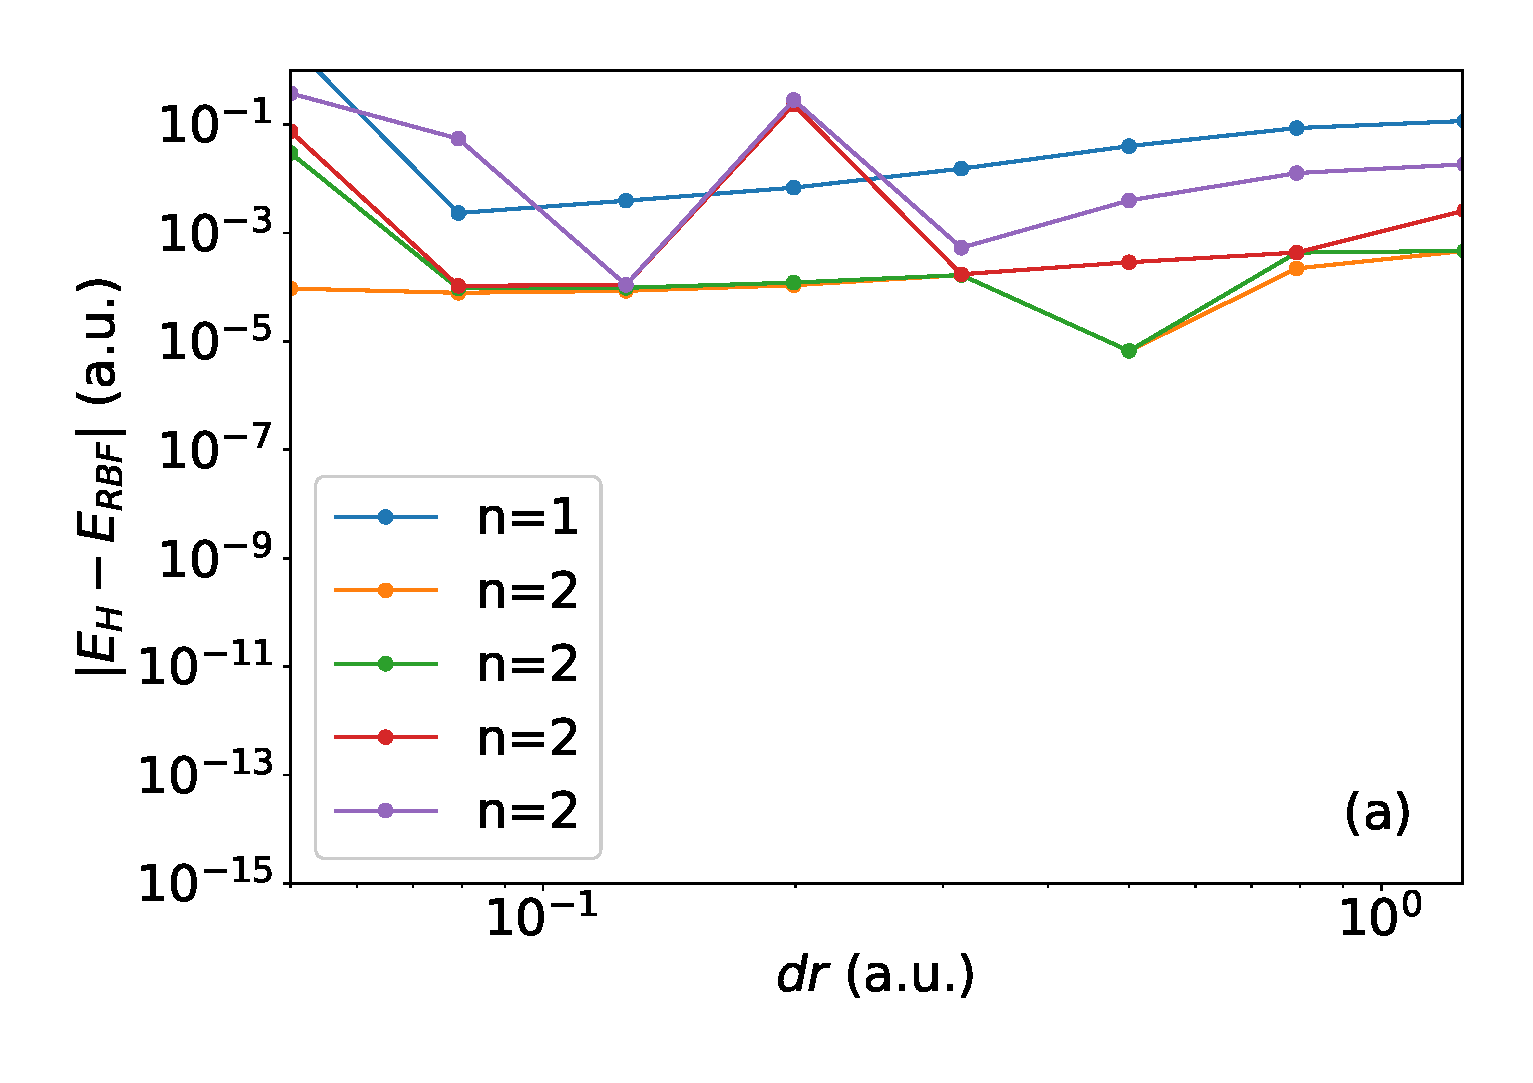
\includegraphics[width=0.32\linewidth]{figs/rbf_no_exp.eps}
    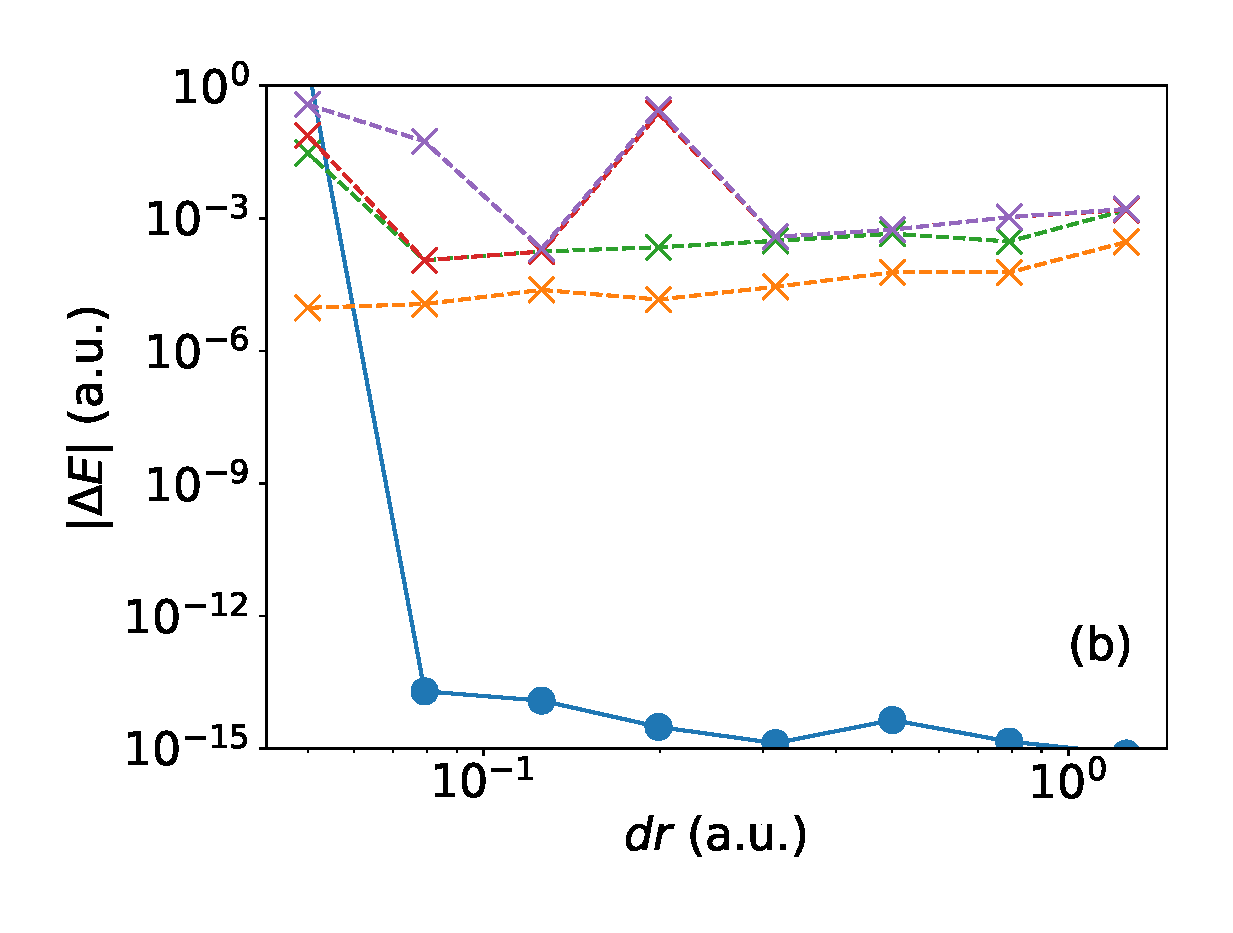
\includegraphics[width=0.32\linewidth]{figs/rbf_with_exp.eps}
    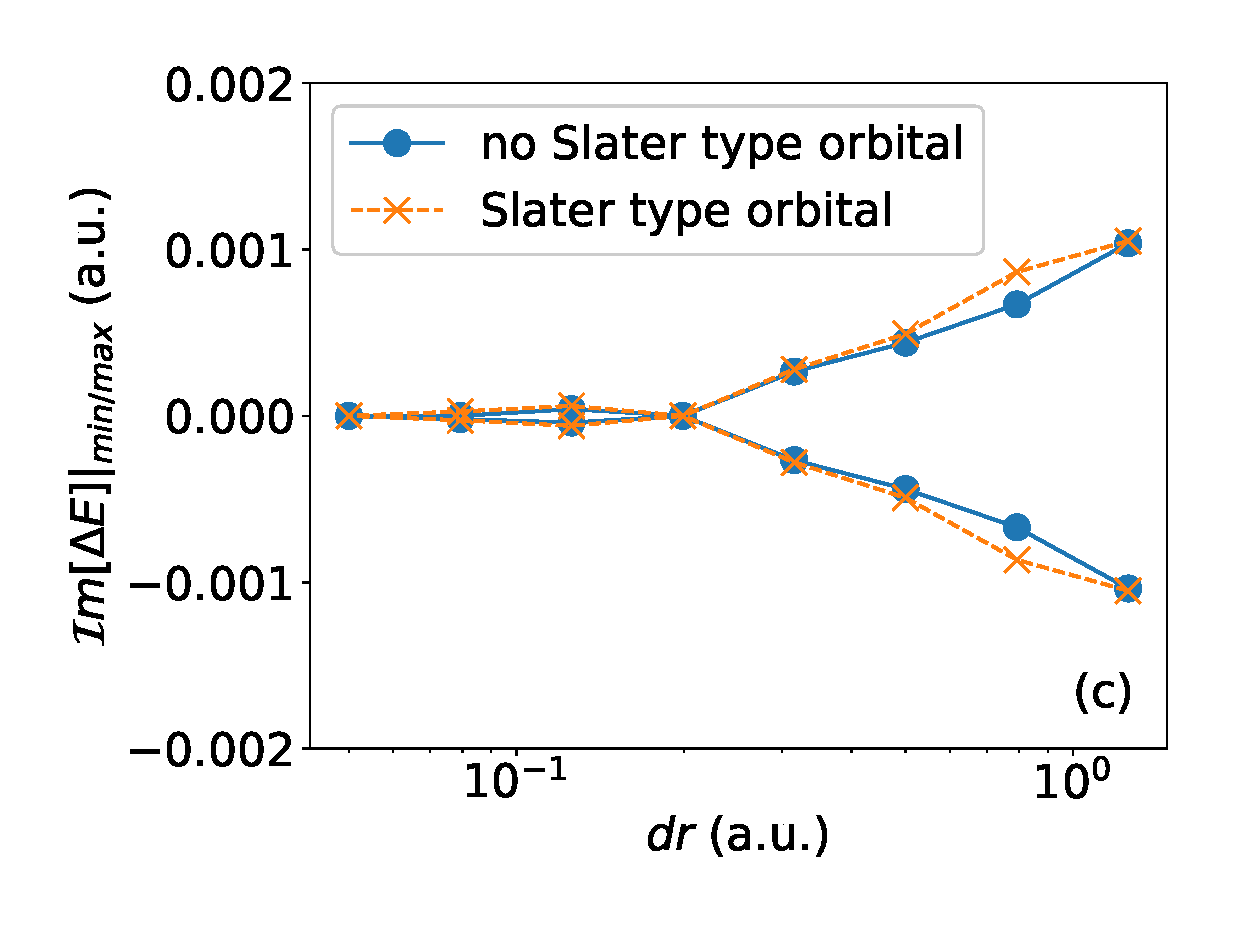
\includegraphics[width=0.32\linewidth]{figs/rbf_imag.eps}
   
\caption{Panels a (b) show the convergence of the lowest energy bound states in Hydrogen without (with) an attached Slater type orbital for various radial spacing ($dr$). Panel c shows the minimum and maximum imaginary part of the calculated bound state energies.
} 
  \label{fig:rbf_conver}
\end{figure}

Convergence of the lowest 5 bound states using the RBF code are shown in Fig.~\ref{fig:rbf_conver}. Results were obtained on mesh with a 30 a.u.\ radial extend, 8th order MD node set, 7th order PHS RBF, attached polynomials up to 3rd order, and a stencil size of 54 nodes. Panel a and b shows the error in the real part of the states energy without and with a Slater type orbital $e^{-r}$ being attached. The addition for the Slater type orbital give machine precision for the ground state (blue line) and improves the 2s (orange line) energy until nonphysical states appear with $dr<0.1$. The 2p states see little benefit from the Slater type orbital.

Fig.~\ref{fig:rbf_conver}c shows the maximum and minimum imaginary part of the energy of the 5 calculated states. The splitting occurs for the states with $m\ne0$ when meshes other than a Cartesian  lattice are used. The states with $\mathcal{I}m[E]<0$ lead to unstable time propagation for the Crank-Nicolson method used in this work. Further work on mesh generation, Hyperviscoisty, and/or time propagation methods will be needed to study time dependent problems with the RBF.


% subsection radial_basis_functions (end)

\subsection{Numerical integration} % (fold)
\label{sub:numerical_integration}
For the finite difference integration, either the midpoint or trapezoid rule are used for numerical integration. For both methods the integration is performed by 
\begin{equation}
    \int_{x} f(x')dx' = \sum_{i=1}^n c_i f(x_i)
\end{equation}
where $f(x_i)$ is the value of the function at $x_i$ and $x$ is the integration interval. The midpoint rule is used if the grid is placed at half grid points on the interval (i.e. $x_i = (2i+1)dx/3$ for $i=0,1,2,...,n$). In this case $c_i = 1/dx$ for all grid points. For the trapezoid rule the grid points sample the ends of the integration range resulting in $c_0 = c_n = 1/2dx$ and $c_i = 1/dx$ for $i=1, ldots, n-1$. 

In the case of the RBF code, the MD node set comes with a provided integration weight for the angular integration and the radial integration is done via the midpoint rule. 
For the spherical code, the angular integration is done analytically since spherical harmonics are orthonormal.
% subsection numerical_integration (end)

\subsection{Boundary conditions} % (fold)
\label{sub:boundary_conditions}
The wavefunction at large $r$ must decay to zero for it to be normalizable. Therefore, we set the wavefunction to zero at $r_{max}$ and increase the value of $r_{max}$ until a converged result is obtained (Sec.~\ref{sub:convergence_studies}). Exterior complex scaling (ECS), which is discussed in the next paragraph, insures that the wavefunction decays prior to hitting the boundary. For the Cartesian code, this is the only boundary conditions needed. For the cylindrical and spherical codes, another boundary condition at $r=0$ is required. The cylindrical code the grid is chosen such that the grid points are given by $x_j = (2j+1)dx/2$ with $j=0, 1, 2, \ldots, n$ and the boundary condition of $\psi(-x)=\psi(x)$ is used. In the spherical code, however, $x_j = jdx$ with $j=1,2,3, \ldots, n$ and the boundary condition $\psi(0)=0$ is used. To enforce a boundary condition a ``ghost node'' is implemented. The ghost node is a grid point that falls outside of the grid. If the ghost node is set to zero, the coefficient is left off the matrix, and the boundary condition is met. If the stencil would be extending beyond the grid by more than one point, such as in 4th order finite difference, the stencil is shifted so that only one point is beyond the grid and it retains the same width (see Fig.~\ref{fig:ghost_nodes}). For the cylindrical case, the ghost node is taken at $\psi(-dx/2)$. Since $\psi(-x)=\psi(x)$, the stencil coefficient at $\psi(-dx/2)$ is added to the coefficient for $\psi(dx/2)$ which imposes the boundary condition.

\begin{figure}[t]
\centering
   
    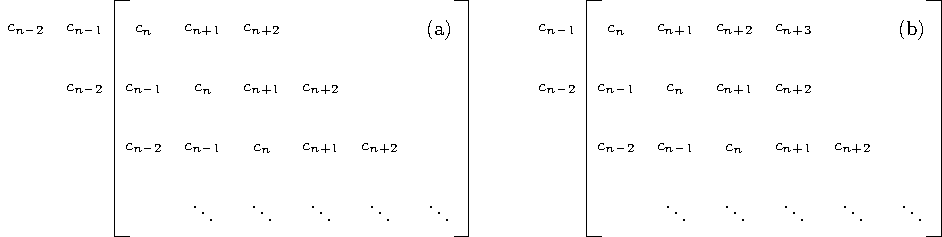
\includegraphics[width=\linewidth]{figs/ghost_nodes.pdf}
   
\caption{The finite difference stencil near the edge of the grid. Panel (a) shows how in the fourth order finite difference the stencil extends beyond the grid leading to a boundary condition being imposed at two points. Panel (b) shows the non-centered 4th order stencil that enforces a single boundary condition.
} 
  \label{fig:ghost_nodes}
\end{figure}


To absorb any outgoing wave packets, we utilize an exterior complex scaling method (ECS, \cite{He_ECS_2007}) on the outer portion of the grid. This is equivalent to changing the spatial step used in finite difference from $x_{n+1} = x_n+dx$ to $x_{n+1} = x_n+e^{i\eta}dx$. In test calculations we have found that $\eta=\pi / 4.0$ works well. The result is an exponential decay of the wavefunction in the absorbing region. Obtaining the finite difference weights in the transition and ECS region is done by implementing the Fornberg method \cite{Fornberg1988} using complex numbers.
% subsection boundary_conditions (end)


\subsection{Bound state calculations} % (fold)
\label{sub:bound_state_calculations}
The bound states of the system are simply the eigenstates of the Hamiltonian with energies less than zero. Therefore they satisfy the equation 
\begin{equation}
    \hat{H} \phi_i = E_i \phi_i
\end{equation}
where $\hat{H}$ is the Hamiltonian, $E_i$ is the energy, and $\phi_i$ is the bound state assuming $E_i < 0$. To solve for the bound states, we use the Krylov-Schur method that is implemented in the SLEPc library \textbf{CITATION NEEDED}. When obtained using SLEPc, the states have a random complex phase associated with them. The phase is physically irrelevant unless one is creating a superposition or comparing the phase of populations between calculations that uses different bound state sets such as a TDSE and PT result. To avoid issues, it is best to use a single bound state calculation for each project. The populations obtained via projections onto excited bound states at the end of a simulation are, for example, useful to analyze and verify selection rules for a given laser polarization.

The coordinate system used for bound state calculations will control which states are generated. For spherical calculations, each $\ell$ block can be calculated independently and the results are independent of $m$. Likewise, results of cylindrical 2D calculations are obtained for fixed $m$ quantum number. Finally, Cartesian 3D calculations will provide all $n$, $\ell$, and $m$ states in one calculation with the states being oriented at a random angle.
% subsection bound_state_calculations (end)

\subsection{Continuum states} % (fold)
\label{sub:continuum_states}
The continuum has states at all levels with energy larger than zero in the physical problem. However, when we solve the TDSE numerically, due to the finite extension of the grid the continuum is represented via a discrete set of states. For example, in spherical coordinates the TDSE solution on the grid requires $\psi(0) = \psi(r_{max}) = 0$ (for the radial coordinate). The same boundary condition is the same as for an infinite square well, however with a bottom in the shape of $V(r)$. The continuum states are therefore a distorted solution to the infinite square well problem. We can obtain these states by the same method as used in the bound state calculations providing a discrete set of energies that represent the continuum. This method is used for the numerical PT solution discussed in Sec.~\ref{sec:perturbation_theory}.

When calculating a photoelectron (energy or angular) spectrum, however, it is advantageous to be able to select the energy of the continuum wave. For this case, we utilize the shooting method to obtain a continuum wave at a given energy. The method is given via an ODE which one solves it as follows. The wavefuction at $r=0$ is set to zero by the boundary condition. The first point at $r_0=dr$ is set to an arbitrary value (in this case 1) giving 
\begin{equation}
    \phi_{kl}(r_0) = 1.
\end{equation}
with $k=\sqrt{2E}$. The second point is then obtained by
\begin{equation}
    \phi_{kl}(r_1) = \phi_{kl}(r_0) \left(dr^2\left[\frac{\ell (\ell+1)}{r^2} + 2V(r_0) -2 E\right]+2 \right). 
\end{equation}
Then every additional point can be found by 
\begin{equation}
    \phi_{kl}(r_{i+1}) = \phi_{kl}(r_i) \left(dr^2\left[\frac{\ell (\ell+1)}{r^2} + 2V(r_i) -2 E\right]+2 \right) - \phi_{kl}(r_{i-1}).
\end{equation}
Now that the wavefunction has been obtained, we match the asymptotic solution to that for a hydrogen-like atom
\begin{equation}
  \phi_{kl}(r\gg1) \rightarrow \sin\left[kr - \frac{l\pi}{2} +\frac{Z}{k} \ln(2kr) + \delta_{kl} \right].
\end{equation}
The continuum state oscillates between -1 and 1 at $r\gg1$ leading to a normalization of
\begin{equation}
  A = \left[\frac{1}{\sqrt{|\phi_{kl}(r)|^2 + \left|\frac{\phi_{kl}'(r)}{(k+\frac{Z}{kr})}\right|^2}} \right]_{r=r_{max}}.
\end{equation}
Finally, we extract the phase shift $\delta_{kl}$ by
\begin{equation}
    \delta_{kl} = \left[Arg\left(\frac{i\phi_{kl}(r) + \frac{\phi_{kl}'(r)}{(k+\frac{Z}{kr})} }{(2kr)^{iZ/k}}\right) - kr + \frac{l\pi}{2} \right]_{r=r_{max}}.
\end{equation}
This continuum state can then be used to obtain the photoelectron spectrum by 
\begin{equation}
    P(k,\theta,\phi) \propto \left|\sum_{l,m} Y_{l,m}(\theta,\phi)\int  e^{-i\delta_{kl}}(i)^l \phi_{kl}(r)^* \psi(r,t) dr \right|^2.
\end{equation}
% subsection continuum_states (end)

\subsection{Time propagation} % (fold)
\label{sub:time_propagation}
Time propagation is often performed using the split-operator method where the Hamiltonian ($\hat{H}$) is split into its spatial dimensions, e.g. along ($z$) and perpendicular ($\rho$) to the polarization direction of a linearly polarized laser. Similarly, the problem can be split along $x$, $y$, and $z$ for an arbitrary laser polarization. The resulting propagation scheme is given by
%
\begin{equation}
    \psi(\mathbf{r},t+\Delta t) \approx e^{-i\hat{H}_{\rho}\frac{\Delta t}{2}} e^{-i\hat{H}_z(t)\Delta t} e^{-i\hat{H}_{\rho}\frac{\Delta t}{2}}\psi(\mathbf{r},t),
     \label{eq:Split-operator}
\end{equation}
%
where
\begin{equation}
    e^{-i\hat{H}\Delta t} \approx \frac{1-i\frac{\Delta t}{2} \hat{H}}{1+i\frac{\Delta t}{2} \hat{H}}.
\end{equation}
This produces a set of tridiagonal matrices which can be solved with $\mathcal{O}(\mathcal{N})$ operations and $\mathcal{O}(\mathcal{N})$ memory. However, parallelization of such a method on a modern supercomputer with distributed memory can be cumbersome, requiring multiple all-to-all Message Passing Interface (MPI) messages during each time step which strongly reduces its scalability.

Instead, we avoid splitting the Hamiltonian and propagate the total Hamiltonian in time using a second order Crank-Nicolson scheme where
%
\begin{equation}
    \psi(\mathbf{r},t+\Delta t) \approx e^{-i\hat{H}\Delta t}\psi(\mathbf{r},t).
    \label{eq:Crank_Nicolson}
\end{equation}
%
We note that the Crank-Nicolson method is not tridiagonal (due to a tensor product) and a direct solution would require $\mathcal{O}(\mathcal{N}^3)$ operations and $\mathcal{O}(\mathcal{N}^2)$ memory which is significantly more than in the split operator method. However, the system of equations in the full Crank-Nicolson method is sparse and iterative methods can be used to vastly accelerate the time propagation. We utilize the Generalized Minimal Residual Method (GMRES), implemented in PETSc, which solves the sparse system of linear equations in $\mathcal{O}(\mathcal{N}\log(\mathcal{N}))$ operations and $\mathcal{O}(\mathcal{N})$ memory. The PETSc library makes it straightforward to parallelize the Crank-Nicolson method on modern supercomputers with distributed memory. On a local supercomputer (Summit, CU Boulder), we achieved super-linear scaling up to 3,000+ cores (see Fig.~\ref{fig:scaling}) allowing us to complete simulations in a matter of hours that would take weeks running on a high-end workstation. 
% subsection time_propagation (end)



\subsection{Convergence studies} % (fold)
\label{sub:convergence_studies}
Numerical solutions to the TDSE require a convergence study to ensure that the final results are reliable. One does this by varying  a free parameter, such as grid spacing, spherical harmonic expansions, time step, etc, until the observable in question changes within some tolerance. It is possible to use an error calculation and reduce it until a numerical tolerance is met. However, graphical convergence, when 2 lines plotted on top of each other are indistinguishable, is often a more practical convergence criteria. In Table~\ref{tab:grid_spacing} we show the error of the ground state energies of a hydrogen-like atom with difference charge ($Z$) converges with grid spacing when using 4th order finite difference.
\begin{table}[t]
\begin{center}
\begin{tabular}{|c|c|c|c|c|c|}
\hline
dx & Z=1 & Z=2 & Z=3 & Z=4 & Z=5 \\ \hline
4.000e-01 & 5.995e-03 & 6.217e-02 & 1.590e-01 & 2.568e-01 & 3.416e-01\\ \hline
2.000e-01 & 3.035e-04 & 5.995e-03 & 2.612e-02 & 6.217e-02 & 1.086e-01\\ \hline
1.000e-01 & 1.041e-05 & 3.035e-04 & 1.841e-03 & 5.995e-03 & 1.392e-02\\ \hline
5.000e-02 & 2.225e-07 & 1.041e-05 & 7.810e-05 & 3.035e-04 & 8.331e-04\\ \hline
2.500e-02 & -2.663e-09 & 2.225e-07 & 2.290e-06 & 1.041e-05 & 3.204e-05\\ \hline
1.250e-02 & -7.101e-10 & -2.672e-09 & 2.992e-08 & 2.225e-07 & 8.341e-07\\ \hline
\end{tabular}
\end{center}
  \caption{\label{tab:grid_spacing}The relative error of the ground state energy for a hydrogen-like atom with a nuclear charge $Z$. A grid spacing around 0.1 produces well converged results for $Z=1$. Excited states have lower relative error.}
\end{table}

For a fixed target, it is advantageous to use the highest order finite difference that is stable. Fig.~\ref{fig:order_convergence} shows the convergence of the $1s$, $2s$, and $3s$ energy levels of the hydrogen atom using $2^{nd}$ through $20^{th}$ order FD. The slope of the convergence for each curve matches the order of the method. $20^{th}$ order FD achieves a converged result with the largest grid spacing leading to a shorter calculation. It is therefore advantageous for bound state calculations. However, the Hamiltonian for higher order methods become increasingly non-Hermitian near the boundaries leading to unstable time propagation for $6^{th}$ or higher order FD. Therefore, we use $4^{th}$ order for the vast majority of calculations that we have performed in this work.

\begin{figure}[h!]
\centering
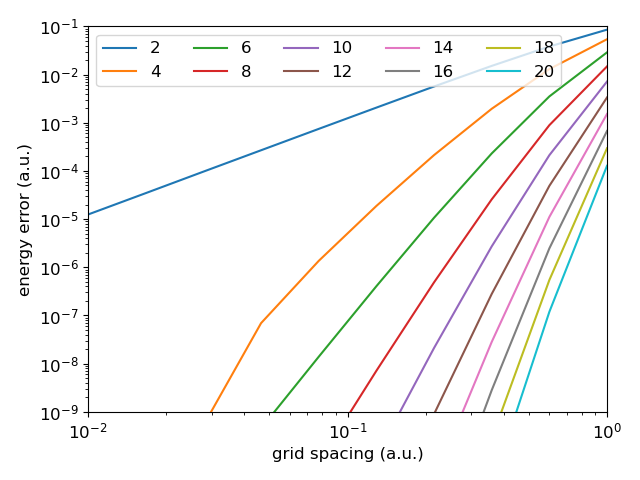
\includegraphics[width=0.32\columnwidth]{figs/1s_conv.png}
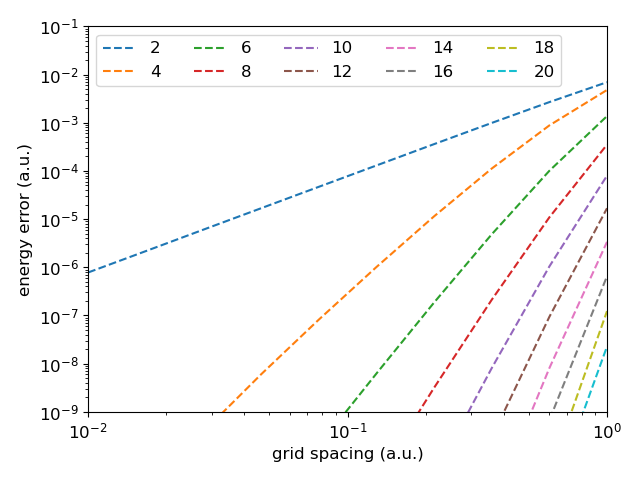
\includegraphics[width=0.32\columnwidth]{figs/2s_conv.png}
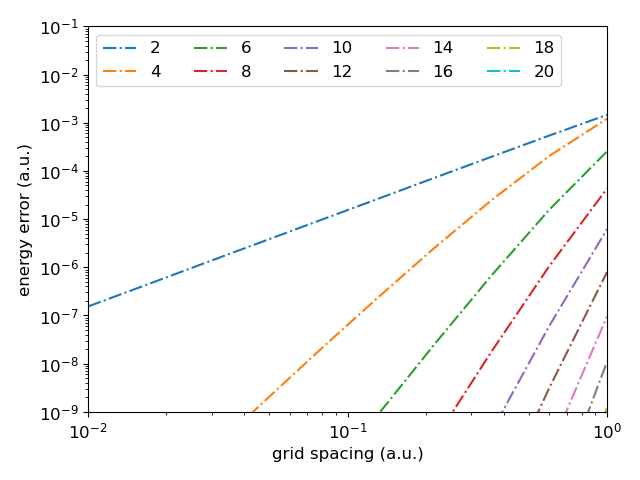
\includegraphics[width=0.32\columnwidth]{figs/3s_conv.png}
\caption{\label{fig:order_convergence} Convergence with respect to grid spacing for various orders of FD for the $1s$ (a), $2s$ (b), and $3s$ (c) states in hydrogen atom.
}
\end{figure}

% subsection convergence_studies (end)
\subsection{Parallel Computing} % (fold)
\label{sub:parallel_computing}
\begin{figure}[h!]
\centering
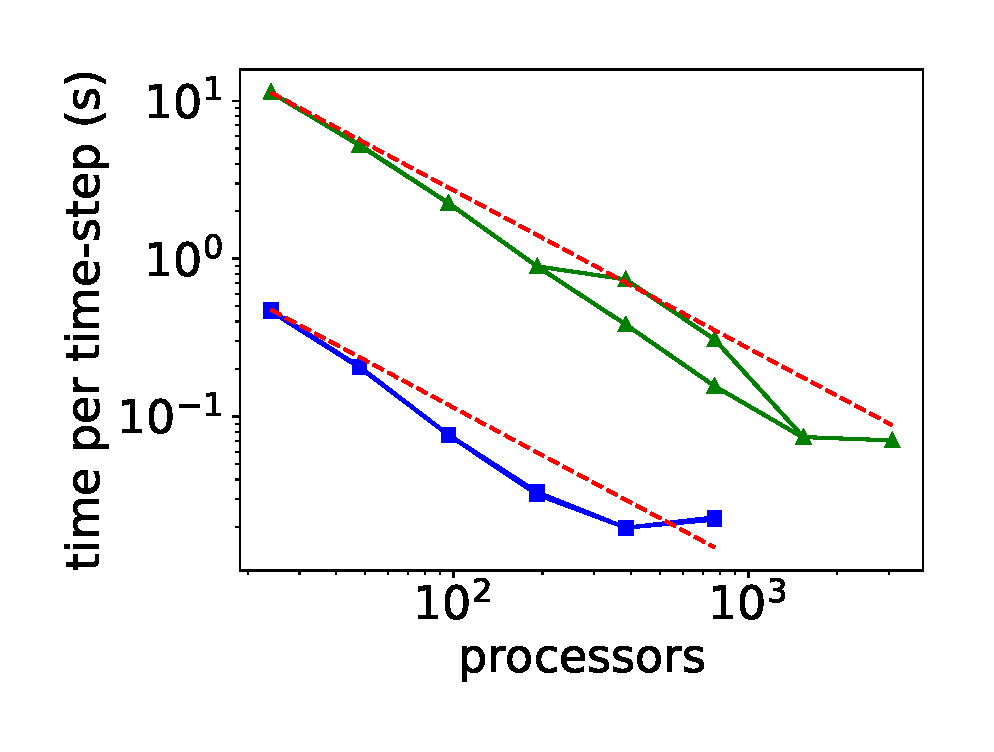
\includegraphics[width=0.5\columnwidth]{figs/Rydberg/multi_node.eps}
\caption{\label{fig:scaling} Scaling results for present Crank-Nicolson method. Two runs each for calculations with 1 million (blue with squares) and 15 million grid points (green with triangles) have been performed. Note that the scaling improves with increasing number of grid points.
}
\end{figure}
Many simulations can be performed on a laptop or small desktop, however, the largest calculations, such as those done in Cartesian coordinates or utilizing bi-circular laser polarizations, benefit from supercomputing resources. Since the code is implemented utilizing the PETSc library and through the use of MPI, we are able to take advantage of the distributed memory of a modern supercomputer. Linear scaling, when the computational time is cut in half when twice as many processors are used, is often the benchmark for code scaling. Our code obtains super-linear (better than linear) scaling on the Summit supercomputer up to 3,000+ processors (see Fig.~\ref{fig:scaling}). This is possible due to the increased size of cache memory as the number of CPUs increases. This allows for calculations that would take a month on a desktop to be completed in a few hours on a supercomputer. Additionally, the supercomputing systems come with a large increase in the available RAM (often on the order of terabytes) significantly reducing the memory limitations on calculation size.

% subsection parallel_computing (end)

% section numerical_methods (end)


%%%%%%%%%%%%%%%%%%%%%%%%%%%%%%%%%%%%%%%%%%%%%%%%%%%%%%%%%%%%%%%%%%%%%%%%%%%%%%%%%%%%%%%%%%%%%%%%%%%%%%%%%%%%%%%%%%
%%%%%%%%%%%%%%%%%%%%%%%%%%%%%%%%%%%%%%%%%%%%%%%%%%%%%%%%%%%%%%%%%%%%%%%%%%%%%%%%%%%%%%%%%%%%%%%%%%%%%%%%%%%%%%%%%%
%%%%%%%%%%%%%%%%%%%%%%%%%%%%%%%%%%%%%%%%%%%%%%%%%%%%%%%%%%%%%%%%%%%%%%%%%%%%%%%%%%%%%%%%%%%%%%%%%%%%%%%%%%%%%%%%%%
%%%%%%%%%%%%%%%%%%%%%%%%%%%%%%%%%%%%%%%%%%%%%%%%%%%%%%%%%%%%%%%%%%%%%%%%%%%%%%%%%%%%%%%%%%%%%%%%%%%%%%%%%%%%%%%%%%
%%%%%%%%%%%%%%%%%%%%%%%%%%%%%%%%%%%%%%%%%%%%%%%%%%%%%%%%%%%%%%%%%%%%%%%%%%%%%%%%%%%%%%%%%%%%%%%%%%%%%%%%%%%%%%%%%%
\section{Single active electron potentials}
\label{sec:SAE}
For many atoms, full treatment of Eq.~\ref{eq:atoms_and_molecules} is impractical if not impossible. Since in many ultrafast laser-atom interactions primarily a single valence electron is involved, in this cases it becomes advantageous to treat only the single active electron in the potential produced by freezing the remaining $N-1$ electrons in their ground state reducing the problem from $3^N$-dimensions down to 3-dimension. The resulting Hamiltonian becomes
\begin{equation}
  \label{eq:SAE_TDSE}
  \hat{H} = -\frac{\mathbf{p}^2}{2} + V_{SAE}(\mathbf{r}) + V_{las}(t)
\end{equation}
where $V_{las}(t)$ is the laser operator and $V_{SAE}(\mathbf{r})$ is the SAE potential. The SAE potentials utilized in this work take the form \cite{reiff_single-active_2020} 
\begin{equation}
  \label{eq:SAE_pot}
  V_{SAE}(\mathbf{r}) = - \frac{z}{r} - \frac{Z_c e^{-c r}}{r} - \sum_n a_n e^{-b_n r}.
\end{equation}
The coefficients are obtained by fitting to a potential obtained through density functional theory (DFT).  In tab.~\ref{tab:SAE} we show the coefficients for SAE potentials used in this thesis.
\begin{table}
\begin{center}
 \begin{tabular}{|c|c|c|c|c|c|c|c|} 
 \hline
 \textbf{Atom} & $z$ & $Z_c$ & $c$ & $a_1$ & $b_1$ & $a_2$ & $b_2$ \\
 \hline
 \textbf{H} & 1 & - & - &  - & - &  - & - \\ 
 \hline
 \textbf{He} & 1 & 1 & 2.0329 &  0.3953 & 6.1805 &  - & - \\ 
 \hline
 \textbf{Ne} & 1 & 9 & 0.8870 &  -9.9286 & 1.3746 &  -5.9950 & 3.7963 \\ 
 \hline
\end{tabular}
\end{center}
 \caption{Coefficients of SAE potentials in Eq.~\ref{eq:SAE_pot} for hydrogen, helium, and neon from \cite{reiff_single-active_2020}.}
 \label{tab:SAE}
\end{table}


%%%%%%%%%%%%%%%%%%%%%%%%%%%%%%%%%%%%%%%%%%%%%%%%%%%%%%%%%%%%%%%%%%%%%%%%%%%%%%%%%%%%%%%%%%%%%%%%%%%%%%%%%%%%%%%%%%
%%%%%%%%%%%%%%%%%%%%%%%%%%%%%%%%%%%%%%%%%%%%%%%%%%%%%%%%%%%%%%%%%%%%%%%%%%%%%%%%%%%%%%%%%%%%%%%%%%%%%%%%%%%%%%%%%%
%%%%%%%%%%%%%%%%%%%%%%%%%%%%%%%%%%%%%%%%%%%%%%%%%%%%%%%%%%%%%%%%%%%%%%%%%%%%%%%%%%%%%%%%%%%%%%%%%%%%%%%%%%%%%%%%%%
%%%%%%%%%%%%%%%%%%%%%%%%%%%%%%%%%%%%%%%%%%%%%%%%%%%%%%%%%%%%%%%%%%%%%%%%%%%%%%%%%%%%%%%%%%%%%%%%%%%%%%%%%%%%%%%%%%
%%%%%%%%%%%%%%%%%%%%%%%%%%%%%%%%%%%%%%%%%%%%%%%%%%%%%%%%%%%%%%%%%%%%%%%%%%%%%%%%%%%%%%%%%%%%%%%%%%%%%%%%%%%%%%%%%%
\section{Observables} % (fold)
\label{sec:observables}

The wavefunction, as numerical solution of our calculations, is not experimentally observable, it is therefore necessary to extract experimentally relevant information via observables. For a given observable $\hat{O}$, the expectation value is obtained by calculating $\bra{\Psi}\hat{O}\ket{\Psi}$. In this work we have studied high order harmonic generation (HHG) spectra, ionization, bound state populations, and photo ionization (energy and angular) distributions.

HHG spectra are obtained by first calculating the dipole acceleration using the Ehrenfest theorem
\begin{equation}
  \hat{a}_j =  \frac{\partial V(\mathbf{r})}{\partial j}
\end{equation}
where $j \in x, y, z$ are the Cartesian coordinates. For the hydrogen atom, $\hat{a}_j=j/r^3$ where r is the distance from the nucleus. Then the HHG spectrum is obtained by taking a Fouirier transform such that
\begin{equation}
    \hat{O}_{HHG}(\omega)_j = \left| \int_{-\infty}^\infty e^{-i2\pi\omega t}\bra{\Psi(t)}\hat{a}_j\ket{\Psi(t)}dt\right|^2
\end{equation}
Bound state populations are obtained using 
\begin{equation}
  P_{\phi_i} = \left|\bra{\phi_i}\ket{\Psi}\right|^2
\end{equation}
where $\phi_i$ is the field free bound state and $\Psi$ is the wavefunction.

At the beginning of each simulation, the wavefunction is normalized to 1 such that
\begin{equation}
\bra{\Psi(t_0)}\ket{\Psi(t_0)} = 1
\end{equation}
Ionization can then be calculated in two manners. First is by time propagating after the pulse and allowing the ionized wave function to be absorbed by the ECS. Ionization is then obtained by taking 
\begin{equation}
  P_{ion}=1-|\bra{\Psi}\ket{\Psi}|^2
\end{equation}
since $\bra{\Psi(t_0)}\ket{\Psi(t_0)}=1$. This method is slow to converge and susceptible to numerical round off error due to extended time propagation. The preferred method for calculating ionization is 
\begin{equation}
  P_{ion}=1-\sum\limits_i\left|\bra{\phi_i}\ket{\Psi}\right|^2
\end{equation}
where $\phi_i$ is a bound state and the sum over $i$ includes all states the grid supports with a real part of the energy that is less than zero. Therefore the ionization probability can be taken at the end of the pulse reducing the computational expense and numerical error.


The photoelectron spectrum (energy and angular) can are obtained at the end of the pulse by calculating
\begin{equation}
    P(k,\theta,\phi) \propto \left|\sum_{l,m} Y_{l,m}(\theta,\phi)\int  e^{-i\delta_{kl}}(i)^l \phi_{kl}(r)^* \psi(r,t) dr \right|^2
\end{equation}
where $\phi_{kl}(r)$ is a continuum wave, $\delta_{kl}$ is a phase shift, and $Y_{l,m}(\theta,\phi)$ is a spherical harmonic. The angular distribution is obtained by plotting the angular dependence ($\theta$ and $\phi$) for a given energy. The energy distribution is obtained by integrating over $\theta$ and $\phi$. See Sec~\ref{sub:continuum_states} for details on obtaining $\phi_{kl}(r)$ and $\delta_{kl}$.
% subsubsection photo_electron_distributions (end)

% subsection observables (end)


%%%%%%%%%%%%%%%%%%%%%%%%%%%%%%%%%%%%%%%%%%%%%%%%%%%%%%%%%%%%%%%%%%%%%%%%%%%%%%%%%%%%%%%%%%%%%%%%%%%%%%%%%%%%%%%%%%
%%%%%%%%%%%%%%%%%%%%%%%%%%%%%%%%%%%%%%%%%%%%%%%%%%%%%%%%%%%%%%%%%%%%%%%%%%%%%%%%%%%%%%%%%%%%%%%%%%%%%%%%%%%%%%%%%%
%%%%%%%%%%%%%%%%%%%%%%%%%%%%%%%%%%%%%%%%%%%%%%%%%%%%%%%%%%%%%%%%%%%%%%%%%%%%%%%%%%%%%%%%%%%%%%%%%%%%%%%%%%%%%%%%%%
%%%%%%%%%%%%%%%%%%%%%%%%%%%%%%%%%%%%%%%%%%%%%%%%%%%%%%%%%%%%%%%%%%%%%%%%%%%%%%%%%%%%%%%%%%%%%%%%%%%%%%%%%%%%%%%%%%
%%%%%%%%%%%%%%%%%%%%%%%%%%%%%%%%%%%%%%%%%%%%%%%%%%%%%%%%%%%%%%%%%%%%%%%%%%%%%%%%%%%%%%%%%%%%%%%%%%%%%%%%%%%%%%%%%%
\section{Laser pulses} % (fold)
\label{sec:laser_pulses}
In order to satisfy Maxwell's equations, the electric field of a laser pulse must integrate to zero. It is therefore convenient to set the vector potential $A(t)$ such that 
\begin{equation}
    A(t) = \frac{c E_0}{\omega_A}f(t) \cos(\omega_A t +\phi_A)
\end{equation}
where $E_0=\sqrt{I}$ is the peak electric field amplitude with $I$ is the peak intensity, $c$ is the speed of light, $\omega_A$ is the central frequency of the vector potential, $\phi_A$ is the carrier-to-envelope phase, and $f(t)$ is the envelope function that starts and ends at zero. We often consider $f(t)$ to be a Gaussian or sine squared function. The electric field can then be obtained via
\begin{equation}
\begin{split}
\label{eq:efield}
E(t) =& -\frac{1}{c}\frac{\partial}{\partial t}A(t)
\\
=&E_0f(t) \sin(\omega_A t +\phi_A)
%\\
%&
-\frac{E_0}{\omega_A}\frac{\partial f(t)}{\partial t}
\cos(\omega_A t +\phi_A).
\end{split}
\end{equation}
where the second term forces the time integral of the electric field to be zero and is only large when the envelope varies quickly over a single optical cycle. This is the case in few cycle pulses and those that turn on or off quickly.

%%%%%%%%%%%%%%%%%%%%%%%%%%%%%%%%%%%%%%%%%%%%%%%%%%%%%%%%%%%%%%%%%%%%%%%%%%%%%%%%%%%%%%%%%%%%%%%%%%%%%%%%%%%%%%%%%%
%%%%%%%%%%%%%%%%%%%%%%%%%%%%%%%%%%%%%%%%%%%%%%%%%%%%%%%%%%%%%%%%%%%%%%%%%%%%%%%%%%%%%%%%%%%%%%%%%%%%%%%%%%%%%%%%%%
%%%%%%%%%%%%%%%%%%%%%%%%%%%%%%%%%%%%%%%%%%%%%%%%%%%%%%%%%%%%%%%%%%%%%%%%%%%%%%%%%%%%%%%%%%%%%%%%%%%%%%%%%%%%%%%%%%
%%%%%%%%%%%%%%%%%%%%%%%%%%%%%%%%%%%%%%%%%%%%%%%%%%%%%%%%%%%%%%%%%%%%%%%%%%%%%%%%%%%%%%%%%%%%%%%%%%%%%%%%%%%%%%%%%%
%%%%%%%%%%%%%%%%%%%%%%%%%%%%%%%%%%%%%%%%%%%%%%%%%%%%%%%%%%%%%%%%%%%%%%%%%%%%%%%%%%%%%%%%%%%%%%%%%%%%%%%%%%%%%%%%%%
\subsection{Frequency shift\protect\footnote{The content of this subsection has been also published in J. Venzke et al. PRA \textbf{98}, 063409 (2018)}} % (fold)
\label{sub:frequency_shift}
\begin{figure}[h!]
\centering
   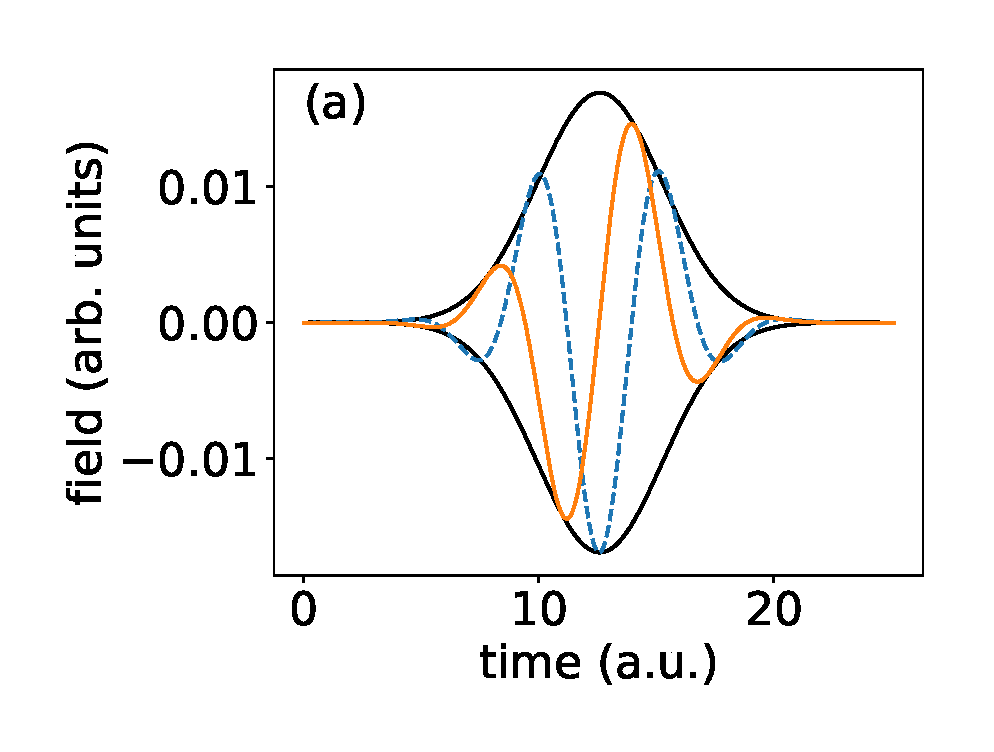
\includegraphics[width=0.35\linewidth]{figs/Frequency_shift/01_field.eps}
   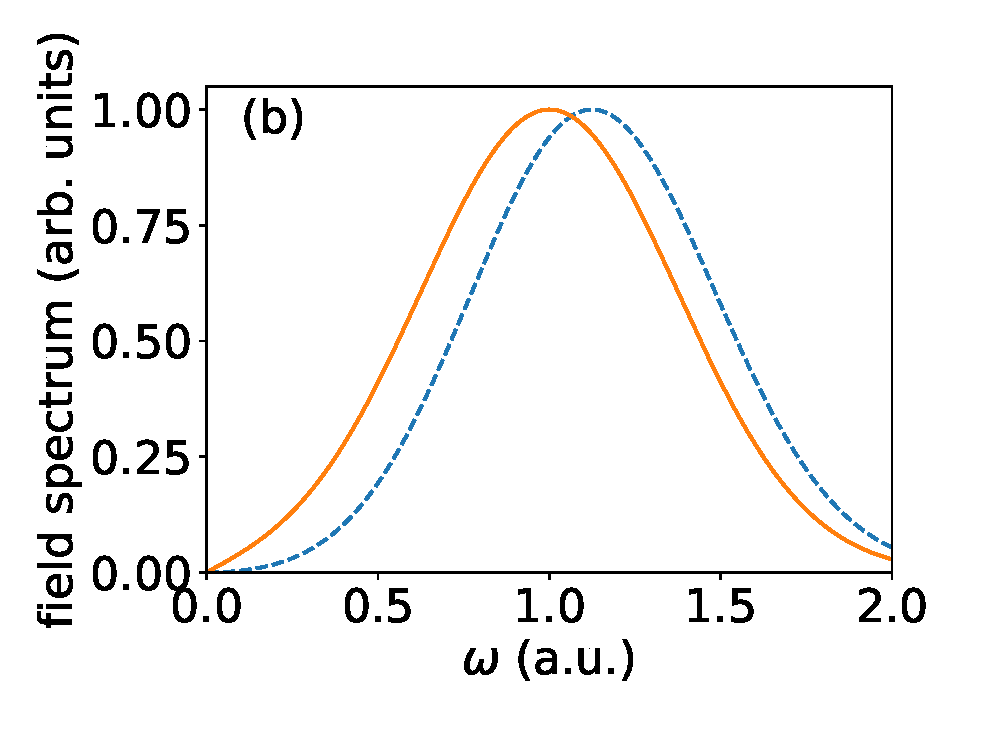
\includegraphics[width=0.35\linewidth]{figs/Frequency_shift/01_spec.eps}
   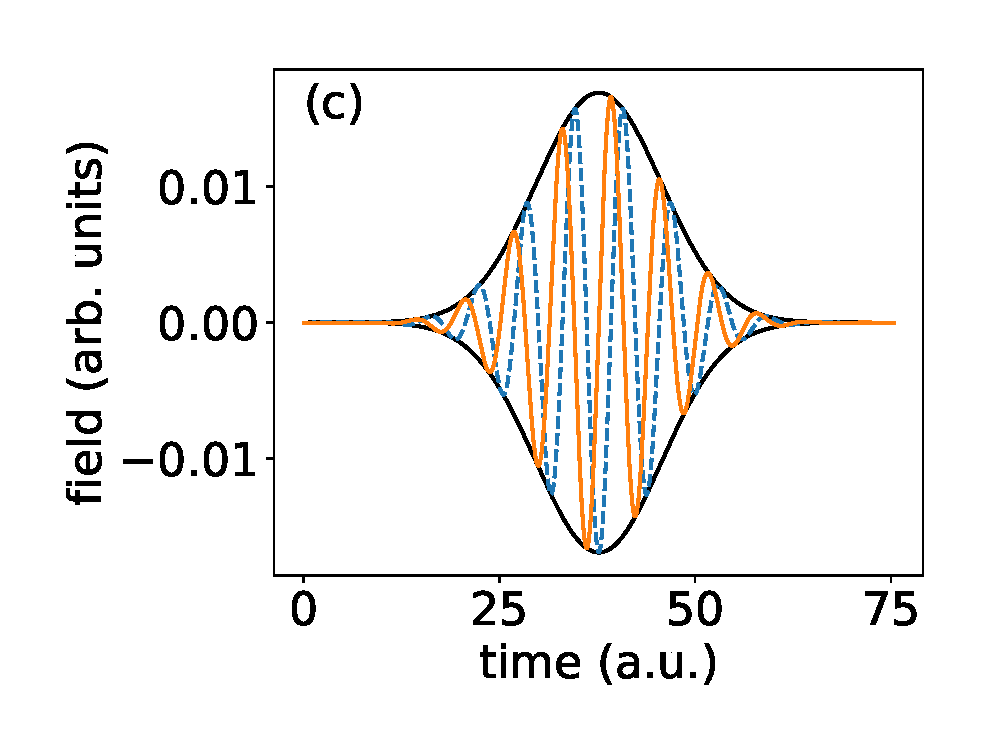
\includegraphics[width=0.35\linewidth]{figs/Frequency_shift/03_field.eps}
   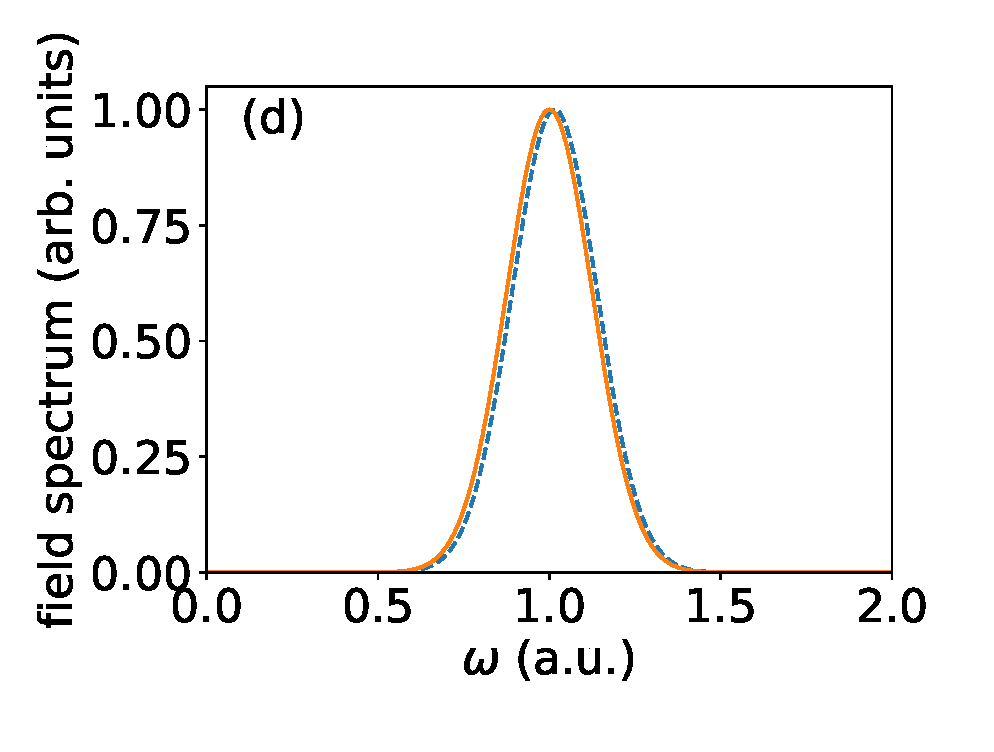
\includegraphics[width=0.35\linewidth]{figs/Frequency_shift/03_spec.eps}
   
\caption{Temporal (left) and spectral (right) distributions of vector potential (solid lines) and electric field (dashed line) for pulses with FWHM of 1 cycle (top), and 3 cycles (bottom) at central frequency $\omega_A = 1.0$ a.u.\  of the vector potential. Also shown is the Gaussian envelope of the vector potential. 
} 
  \label{fig:spectra}
\end{figure}

As the pulse length decreases, the central frequency (defined by the peak of the frequency spectrum) of the vector potential and electric fields differ. In Fig.~\ref{fig:spectra} the dashed blue lines show the electric field and the orange solid lines show the vector potential for a Gaussian pulse with a pulse duration of 1 cycle FWHM (top) and 4 cycle FWHM (bottom). The time domain (right) looks similar, up to the expected $\pi/2$ phase shift, but the frequency spectrum (right) differ significantly for the 1 cycle FWHM pules. By utilizing TDSE solutions, it is possible to show that the central frequency of the electric field is the relevant frequency in both length and velocity gauge calculations \cite{venzke_central_2018}. 
It is, therefore, important to correct the central frequency used in the vector potential when the pulse length is short. An approximate correction is given by
\begin{equation}
\label{eq:fshift}
\frac{\omega_E}{\omega_A} 
\approx
\frac{1+\sqrt{1+4(\pi N)^{-2}}}{2}.
\end{equation}
%
Here
%
\begin{equation}
\begin{split}
\label{eq:nbar}
 N \equiv \frac{\omega_A}{\pi} \sqrt{\frac{\int_{-\infty}^{\infty} (t-t_0)^2 f(t) dt}{\int_{-\infty}^{\infty} f(t) dt}}.
\end{split}
\end{equation}
%
is the number of cycles within one standard deviation to either side of the pulse center, with
%
\begin{equation}
\begin{split}
t_0 \equiv \frac{\int_{-\infty}^{\infty} t f(t) dt}{\int_{-\infty}^{\infty} f(t) dt}.
\end{split}
\end{equation}
This correction is sufficient for most pulse shapes, however, correction terms can be found in \cite{venzke_central_2018}.




\textbf{HERE}


Few-cycle laser pulses are used in many interesting strong-field applications (for reviews, see e.g., \cite{popmintchev10,suzuki14,vrakking14,pazourek15,wang15,xu16}): For example, high-order harmonics and (isolated) attosecond pulses are generated, ultrafast atomic and molecular dynamics as well as charge transfer and exciton dynamics can be induced and time resolved, molecular structure can be imaged on ultrashort time scales, or chemical reactions may be controlled. Therefore, light sources generating ultrashort intense laser pulses in different regions of the spectrum, at extreme ultraviolet \cite{goulielmakis08}, ultraviolet \cite{durfee99}, optical \cite{fork87}, near-infrared \cite{zhou94,nisoli96,nisoli97} and infrared wavelengths \cite{ishii14,pupeza15,li16}, have been developed over the past decades.  The simulation of the time-dependent response of matter to a few-cycle pulse, e.g. via the numerical solution of the corresponding time-dependent Schr\"odinger equation (TDSE), can however crucially depend on the definition of the electric field $E(t)$ used. To achieve quantitative agreement between theory and experiment, the potential issues present in both numerical calculations and experiment must be well understood and minimized.

As pointed out by Chelkowski and Bandrauk \cite{chelkowski02}, the representation of $E(t)$ via an envelope function times a trigonometric function may lead to a non-vanishing potential $A(t)$ at the end of the pulse. This inconsistency can be resolved by first defining the magnitude of the vector potential $A(t)$ as (we use Hartree atomic units: $e = m_e = \hbar =1$) \cite{chelkowski02}: 
\begin{equation}
A(t) = \frac{c E_0}{\omega_A}f(t) \cos(\omega_A t +\phi_A),
\label{eq:vectorpotential}
\end{equation}
where $f$, $\omega_A$, $c$, $E_0$ and $\phi_A$ are the envelope function, central frequency, speed of light, peak electric field amplitude, and carrier envelope phase of the vector potential, respectively.
The prefactors ensure that the peak intensity of the laser field is $I = \tfrac{c}{8\pi}E_0^2$.
The magnitude of the electric field is then obtained via the derivative:
\begin{equation}
\begin{split}
\label{eq:efield}
E(t) =& -\frac{1}{c}\frac{\partial}{\partial t}A(t)
\\
=&E_0f(t) \sin(\omega_A t +\phi_A)
\\
&
-\frac{E_0}{\omega_A}\frac{\partial f(t)}{\partial t}
\cos(\omega_A t +\phi_A).
\end{split}
\end{equation}

The expression for the electric field, Eq.~(\ref{eq:efield}), includes a term that depends on the time derivative of $f$ and, hence, may have significant effects in the case of few-cycle pulses. As we will show below, a direct implication is that the central frequency of the electric field spectrum, $\omega_E$, is not equal to $\omega_A$. The frequency shift $|\omega_E - \omega_A|$ is a purely electromagnetic effect that is directly related to the definition of the electric field via the vector potential given in Eq.\ (\ref{eq:efield}). For long pulses, the frequency shift is small, but it increases as pulse duration decreases. Note, that in experiment typically the central laser frequency of the electric field $\omega_E$ is measured and reported, while in numerical calculations it is useful to define the laser pulse via the vector potential and the related central frequency $\omega_A$. It is therefore important to study what impact, if any, the difference between the central frequencies has on numerical calculations, or on the interpretation of theoretical results. 

By solving the time-dependent Schr\"odinger equation both numerically as well as within perturbation theory,
we show below that theoretical results obtained for linear processes---such as excitation and ionization---involving few-cycle pulses with the same value for the central frequencies $\omega_A$ and $\omega_E$ do not coincide. Furthermore, we find that the frequency shift is also noticeable for nonlinear processes, such as two-photon excitation and high-order harmonic generation, and it scales with the number of photons involved. Our results also demonstrate that it is the central frequency of the electric field $\omega_E$ that is the physical relevant quantity for the interpretation of laser driven quantum mechanical processes. Therefore, the frequency shift should be taken into account when setting the central frequency $\omega_A$ of the vector potential in a numerical calculation or, more generally, a theoretical analysis.

The paper is organized as follows: In Section \ref{sec:pulse}, we present an analytical estimate for the magnitude of the frequency shift, and discuss how to correct for it.
In Section \ref{sec:applications}, we present results of numerical solutions of the time-dependent Schrödinger equation, which illustrate how the frequency shift affects a number of quantum mechanical processes: photoionization, resonant excitation, and high-harmonic generation. We end with a brief summary.


\begin{figure}[t]
\centering
   
    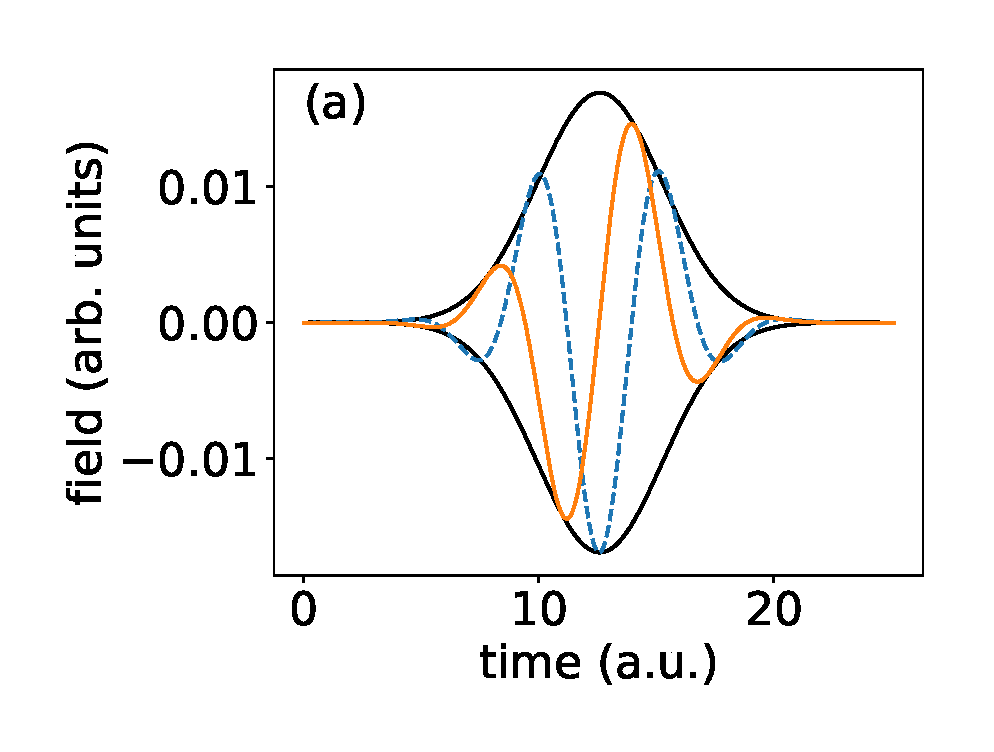
\includegraphics[width=0.49\linewidth]{figs/Frequency_shift/01_field.eps}
    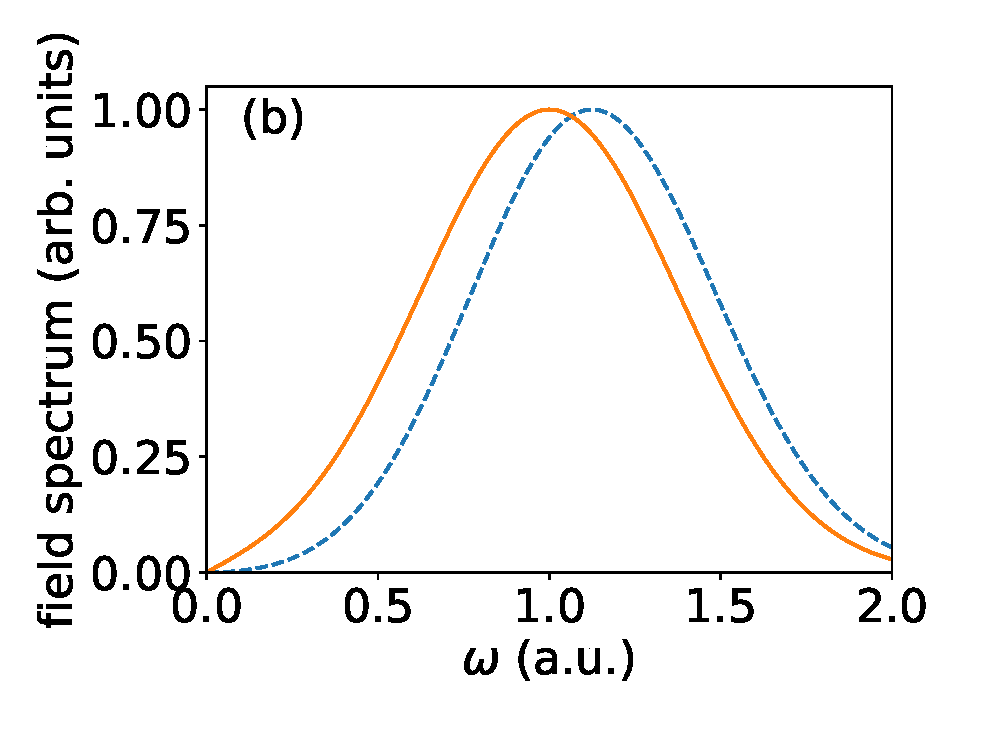
\includegraphics[width=0.49\linewidth]{figs/Frequency_shift/01_spec.eps}
    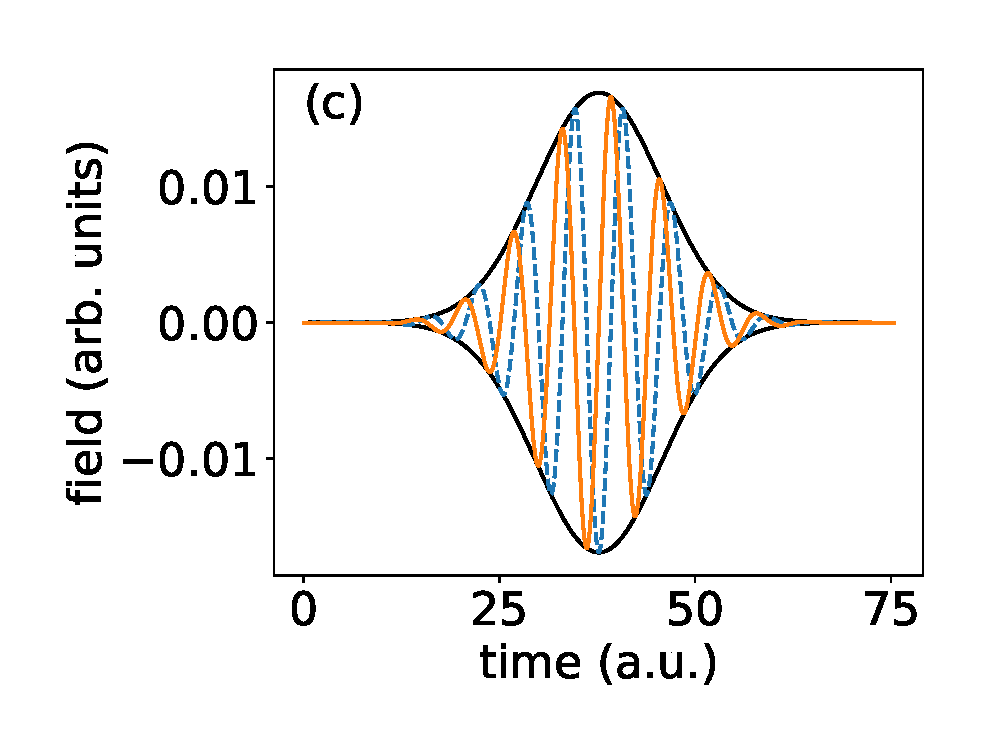
\includegraphics[width=0.49\linewidth]{figs/Frequency_shift/03_field.eps}
    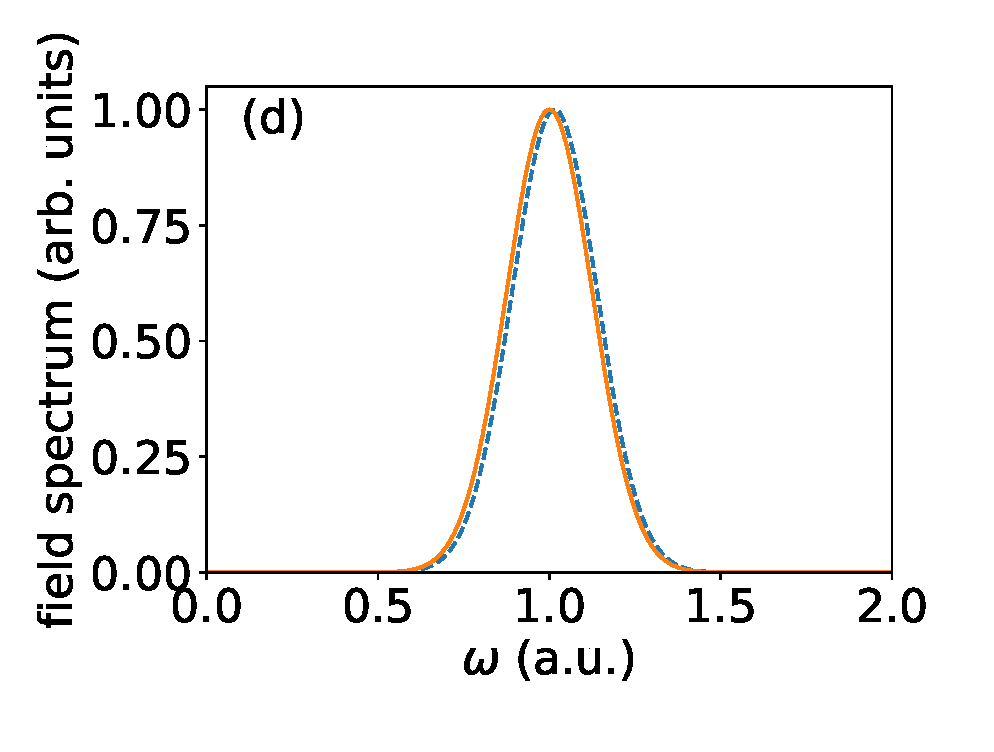
\includegraphics[width=0.49\linewidth]{figs/Frequency_shift/03_spec.eps}
   
\caption{(Color online)
Temporal (left) and spectral (right) distributions of vector potential (solid lines) and electric field (dashed line) for pulses with FWHM of 1 cycle (top), and 3 cycles (bottom) at central frequency $\omega_A = 1.0$ a.u.\  of the vector potential. Also shown is the Gaussian envelope of the vector potential. 
} 
  \label{fig:spectra}
\end{figure}

The frequency shift due to the difference in central frequencies is illustrated in Fig.~\ref{fig:spectra}, where the vector potential $A$ and the electric field $E$, obtained from Eqs. (\ref{eq:vectorpotential}) and (\ref{eq:efield}) for a Gaussian envelope $f(t)$, are compared in both the time and frequency domain. While the temporal behavior is satisfactory, the spectral distributions reveal different central frequencies. We define the central frequency $\omega_A$ ($\omega_E$) as the location of the maximum in the spectral density $|\tilde{A}(\omega)|$ ($|\tilde{E}(\omega)|$). The discrepancy is much greater for the 1-cycle full-width at half-max (FWHM) pulse (top), than for the 3-cycle FWHM pulse (bottom).

\begin{table}
\begin{center}
 \begin{tabular}{||c | c | c | c||} 
 \hline
 Name & Envelope Function $f(t)$ & $ N/N_{\text{FWHM}}$ & $\gamma_2$ \\ [0.5ex] 
 \hline\hline
 Gaussian & $e^{-(t/T)^2}$ & 0.849 & 0 \\ 
 \hline
 Cos$^2$ & $\begin{cases} 
      \cos^2\left(\frac{t}{T}\right) & -\frac{\pi}{2} \leq \frac{t}{T} \leq \frac{\pi}{2} \\
      0 & \text{otherwise}
    \end{cases}$ & 0.723 & -0.594 \\
 \hline
  Cos$^4$ &  $\begin{cases} 
        \cos^4\left(\frac{t}{T}\right) & -\frac{\pi}{2} \leq \frac{t}{T} \leq \frac{\pi}{2} \\
        0 & \text{otherwise}
    \end{cases}$ & 0.777 & -0.381 \\
 \hline
 Sech & $\text{sech}(\frac{t}{T})$ & 1.19 & 2.00 \\
 \hline
\end{tabular}
\end{center}
 \caption{Several common analytic pulse envelopes. The conversion factor between $N$, as defined in Eq.~(\ref{eq:nbar}) (number of cycles within one standard deviation to either side of the maximum), and the more typical $N_{\text{FWHM}}$ (number of cycles in the full-width half-maximum of the electric field) is given. The last column shows the excess kurtosis $\gamma_2$, defined in Eq.~(\ref{eq:gamma2}), which is independent of the pulse duration $T$.}
 \label{tab:envelopes}
\end{table}

For the further analysis, we note that in order for the central frequencies to be well-defined and consistent with the definition of $\omega_A$ in Eq. (\ref{eq:vectorpotential}), we make several assumptions about the envelope $f(t)$:
\begin{itemize}
  \item $f(t)$ is nonnegative and continuously differentiable,
  \item $f(t)$ falls off at least exponentially for large $|t|$, 
\item $f(t)$ contains no appreciable Fourier components larger than $\omega_A$.
\end{itemize}
These assumptions could be relaxed significantly, but they are sufficient for the present discussion and all practical purposes. The ratio of the central frequencies is given by the leading terms of an expansion in $1/N$ as (see Appendix \ref{sec:appendix-frequency}):
\begin{eqnarray}
\label{eq:fshift}
\frac{\omega_E}{\omega_A} 
&=& 
\frac{1+\sqrt{1+4(\pi N)^{-2}}}{2}+ \frac{\gamma_2}{6\pi^4} N^{-4} + O( N^{-6})
\\
\label{eq:fshiftapprox}
&\approx& 
\frac{1+\sqrt{1+4(\pi N)^{-2}}}{2}.
\end{eqnarray}
%
Here
%
\begin{equation}
\begin{split}
\label{eq:nbar}
 N \equiv \frac{\omega_A}{\pi} \sqrt{\frac{\int_{-\infty}^{\infty} (t-t_0)^2 f(t) dt}{\int_{-\infty}^{\infty} f(t) dt}}.
\end{split}
\end{equation}
%
is the number of cycles within one standard deviation to either side of the pulse center, with
%
\begin{equation}
\begin{split}
t_0 \equiv \frac{\int_{-\infty}^{\infty} t f(t) dt}{\int_{-\infty}^{\infty} f(t) dt},
\end{split}
\end{equation}
%
and lastly $\gamma_2$ is the excess kurtosis of the envelope
%
\begin{equation}
\label{eq:gamma2}
\gamma_2 \equiv \frac{\left[\int_{-\infty}^{\infty} (t-t_0)^4 f(t) dt\right]\left[\int_{-\infty}^{\infty} f(t) dt\right]}{\left[\int_{-\infty}^{\infty} (t-t_0)^2 f(t) dt\right]^2}-3.
\end{equation}
%
Note that $N$ is proportional to the more typical $N_{\text{FWHM}}$ (number of cycles in the FWHM of $f(t)$), but the ratio $N/N_{FWHM}$ depends on the shape of the envelope (c.f., Table \ref{tab:envelopes}). 

\begin{figure}[t]
\centering
    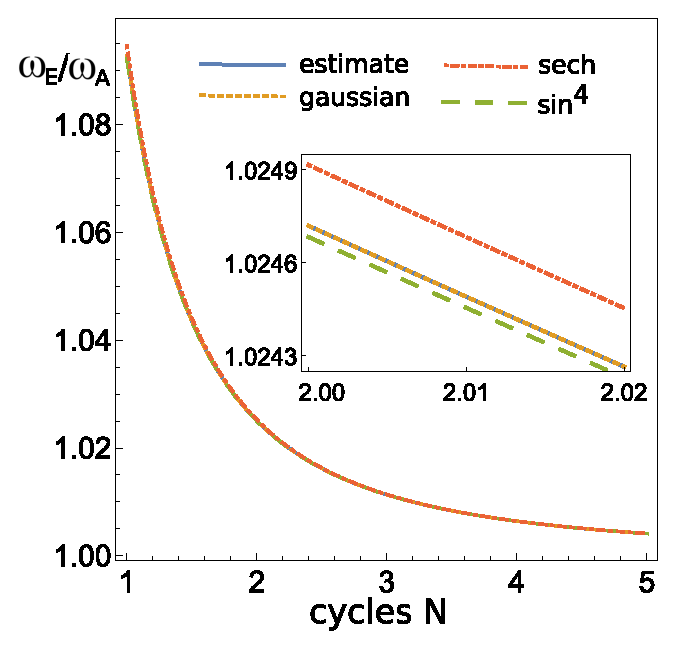
\includegraphics[width=0.8\linewidth]{figs/Frequency_shift/fshift51.eps}
\caption{(Color online)
Ratio $\omega_E/\omega_A$ as a function of the normalized number of cycles $ N$ defined in Eq.~(\ref{eq:nbar}). The numerical results were calculated by maximizing $\tilde{E}(\omega)$ for Gaussian (dotted line), $\text{sech}$ (dashed-dotted line), and $\sin^4$ (dashed line) envelopes and are compared with the simple analytic estimate (solid line) given in Eq.~(\ref{eq:fshiftapprox}). The inset reveals a slight dependence on envelope shape, which can be attributed to the correction term in Eq.~(\ref{eq:fshift}).
}
  \label{fig:shift}
\end{figure}

Eq.~(\ref{eq:fshift}) indicates that the ratio $\omega_E/\omega_A$ depends on the number of cycles and the pulse shape, but it is independent of peak intensity, carrier envelope phase, ellipticity, and $\omega_A$ itself. In fact, the first term of the expansion, Eq.~(\ref{eq:fshiftapprox}), is a very accurate estimate even for single cycle pulses, showing that the shift is nearly independent of pulse shape. This can be seen from the comparison between the predictions based on Eq.~(\ref{eq:fshiftapprox}) with the exact frequency shift for a variety of pulse shapes in Fig.~\ref{fig:shift}. The exact shift was calculated by numerically maximizing the analytic expressions for $|\tilde{E}(\omega)|$. The slight dependence on pulse shape is visible in the inset; the differences are described well by the correction term in Eq.~(\ref{eq:fshift}), which involves the excess kurtosis $\gamma_2$.

In the next section, we demonstrate that $\omega_E$ is the physically observable and relevant central frequency. Therefore, when modeling the interaction with a pulse using Eqs.~(\ref{eq:vectorpotential}) and (\ref{eq:efield}), one should determine $\omega_A$  such that it corresponds to the correct $\omega_E$. There are two different methods to do this. The first one is to specify $N$, and use Eq.~(\ref{eq:fshiftapprox}) to obtain $\omega_A$. However since $N$ depends implicitly on $\omega_A$ through Eq.~(\ref{eq:nbar}), the envelope $f(t)$ must be stretched in time by the same factor such that $N$ remains unchanged. The second method is to specify $f(t)$ instead of $N$. In that case, substituting Eq.~(\ref{eq:nbar}) into Eq.~(\ref{eq:fshiftapprox}) and solving for $\omega_A$ yields
%
\begin{equation}
\label{eq:alternative}
\omega_A \approx \omega_E - \frac{\int_{-\infty}^{\infty} f(t) dt}{\omega_E\int_{-\infty}^{\infty} (t-t_0)^2 f(t) dt}.
\end{equation}
%
Greater accuracy could be obtained in either case by including the correction term in Eq. (\ref{eq:fshift}); however, the results in Fig.~\ref{fig:shift} show that this is in general not necessary. 

In this section we present results of numerical calculations and first-order perturbation theory which exemplify effects of the frequency shift on observables related to excitation, ionization and high harmonic generation induced by short laser pulses. The frequency shifts obtain using first-order perturbation theory and numerical calculations agree well with our analytical predictions shown in Section~\ref{sec:pulse} and derived in Appendix~\ref{sec:appendix-frequency}. To this end, we solved the 3D one-electron time-dependent Schr\"odinger equation (TDSE) in velocity gauge:
\begin{equation}
i\frac{\partial}{\partial t}\psi(\mathbf{r},t) = \left[\frac{\mathbf{p}^2}{2} - \frac{\mathbf{A}(t) \cdot \mathbf{p}}{c} + V(\mathbf{r})\right]\psi(\mathbf{r},t)
\end{equation}
and length gauge
\begin{equation}
i\frac{\partial}{\partial t}\psi(\mathbf{r},t) = \left[\frac{\mathbf{p}^2}{2} + \mathbf{E}(t) \cdot \mathbf{\mathbf{r}} + V(\mathbf{r})\right]\psi(\mathbf{r},t)
\end{equation}
for atomic hydrogen with a soft-core Coulomb potential
\begin{equation}
V(\mathbf{r}) = -\frac{1}{\sqrt{\mathbf{r}^2+\alpha ^2}}.
\end{equation}
We consider a linearly polarized laser pulse within the dipole approximation, so $\mathbf{A}(t)=A(t)\hat{z}$ and $\mathbf{E}(t)=E(t)\hat{z}$. Taking advantage of azimuthal symmetry, the wavefunction can be represented in 2D cylindrical coordinates $\rho$ and $z$. We used the second order finite difference method for spatial derivatives and the fully implicit second order Crank-Nicholson method for time propagation (for more details on the numerical implementation, see \cite{venzke-submitted}). The laser field magnitudes $A(t)$ and $E(t)$ were defined as in Eq.~(\ref{eq:vectorpotential}) and Eq.~(\ref{eq:efield}), with a Gaussian envelope function $f(t)$.
Specifically,
\begin{equation}
\label{eq:numericalVecPot}
A(t) = \frac{E_0c}{\omega_A}\sin(\omega_A t)e^{-(2t/\tau)^2\ln 2} ~,
\end{equation}
where $\tau$ is the FWHM pulse duration. The results presented below were obtained in velocity gauge, but additional test calculations in length gauge have confirmed that the results are gauge invariant.

In all calculations for single photon ionization (Sec.~\ref{sec:single_photon}), excitation (Sec.~\ref{sec:excitation}) and high harmonic generation (Sec.~\ref{sec:HHG}) we used $\alpha=0.029$ a.u.,\ a grid spacing of 0.1 a.u.,\ and a time step of 0.1 a.u. The soft core parameter is used to match the ground state energy to that of atomic hydrogen, given by $E_{1s} = -0.5001$ a.u. on the grid, and an excited state energy of $E_{2p} = -0.12504$ a.u.\  To ensure the wavefunction remains on the grid for our calculation of the photoelectron spectrum, the grid extended 500 a.u.\  in the $\rho$-direction and 1000 a.u in the $z$-direction, with an exterior complex scaling absorbing boundary in the outer 50 a.u for single photon ionization (Sec.~\ref{sec:single_photon}). The excitation (Sec.~\ref{sec:excitation}) and high harmonic generation (Sec.~\ref{sec:HHG}) calculations were preformed on a grid that extended over 100 a.u.\  in the $\rho$-direction and 200 a.u.\ in the $z$-direction, with an absorbing boundary over the outer 5 a.u.

First, we consider single photon ionization of the hydrogen atom by a few-cycle laser pulse with peak intensity $10^{13}$ W/cm$^2$ and central frequency $\omega_{\text{central}} = 2.0$ a.u. The central frequency is implemented either by setting $\omega_A=\omega_{\text{central}}$ or setting $\omega_E=\omega_{\text{central}}$, using the method described in the previous section. Photoelectron momentum spectra $P(k)$ were obtained by the following procedure: the TDSE was propagated for five times the FWHM pulse duration plus an additional 100 a.u.\  in time, then all bound states with principle quantum number $n\le 8$ were projected out, and lastly the remaining unbound wavepacket $\psi_{\text{ionized}}$ was projected onto coulomb wave functions up to $l_{\text{max}}=5$. That is,
%
\begin{equation}
P(k) = \sum_{l=0}^{l_{\text{max}}} \left|\int F_{l}(-\tfrac{1}{k}, kr)Y^*_{l0}(\hat{r})\psi_{\text{ionized}}(\vec{r})d^{3}\vec{r}~\right|^2 ~.
\end{equation}


\begin{figure}[t]
\centering
    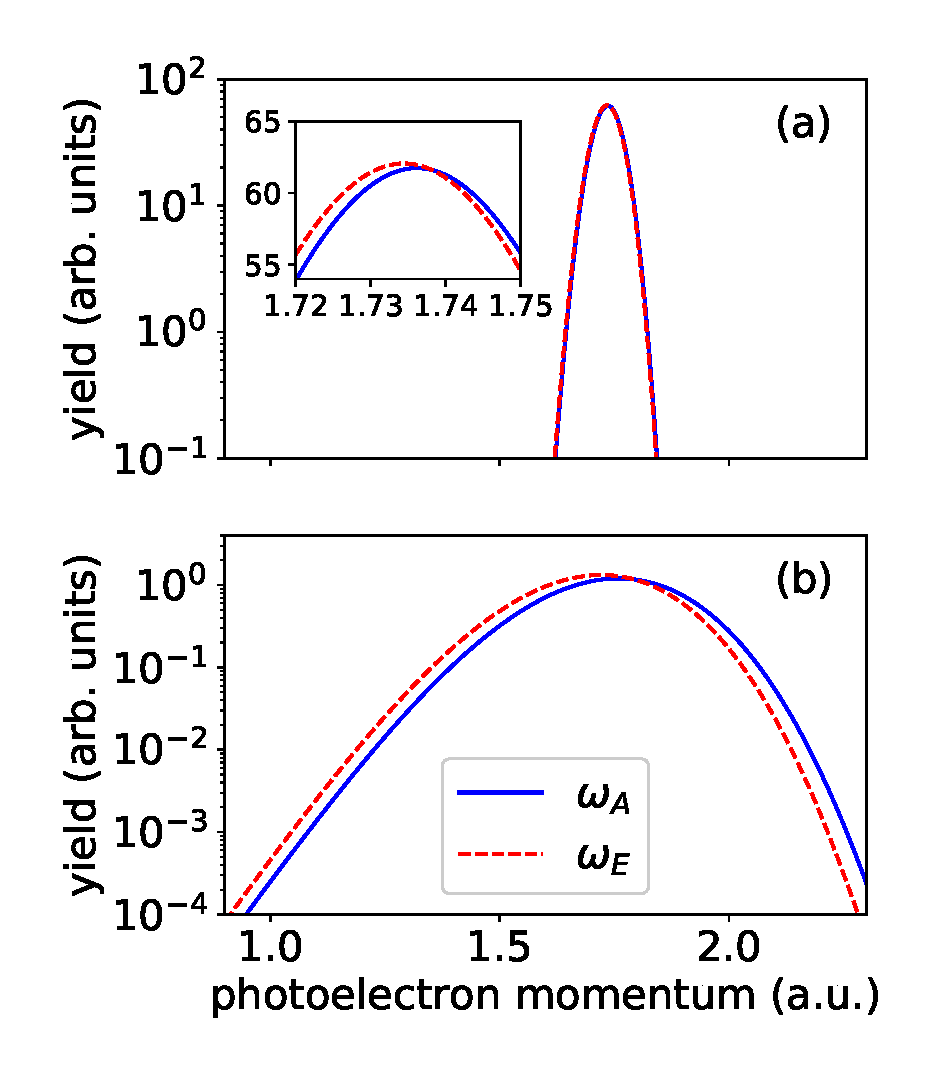
\includegraphics[width=0.8\linewidth]{figs/Frequency_shift/single_photon_ion.eps}
\caption{(Color online)
Photoelectron spectra $P(k)$ as function of photoelectron momentum obtained for interaction of hydrogen atom with laser pulses at central frequencies $\omega_A=2$ (dashed line) and $\omega_E=2$ (solid line) and duration of (a) 10 cycles and (b) 2 cycles FWHM.
}
  \label{fig:ionizationA}
\end{figure}

The results in Fig.~\ref{fig:ionizationA} show that in fact the photoelectron spectra for central frequency $\omega_A = 2$ a.u.\  (solid lines) and $\omega_E = 2$ a.u.\  (dashed lines) do not agree due to the frequency shift. As expected, the discrepancy is larger for 2 cycle FWHM (panel (b)) than for 10 cycle FWHM (panel (a)) pulses. These results however raise the question whether the central frequency of the vector potential $\omega_A$ or the central frequency of the electric field $\omega_E$ is the relevant quantity for further physical interpretation or a comparison with experimental data. To address this question, we consider the resonant population transfer between bound states by analyzing results of numerical calculation as well as those obtained using first-order perturbation theory in the next subsection.

Next, we examine transitions to the $n=2$ orbitals in the hydrogen atom as a function of both pulse length and central frequency of the vector potential ($\omega_A$) and the electric field ($\omega_E$).
Typically, the excitation probability is greatest when the central frequency of the laser matches the resonant frequency for $n_p$ photon absorption, given by
\begin{equation}
\omega_{\text{res}} = |E_\text{final} - E_\text{initial}|/n_p,
\end{equation}
where $E_\text{final}$ and $E_\text{initial}$ are the energy of the final and initial state, respectively. In view of the predicted frequency shift between the central frequencies $\omega_A$ and $\omega_E$, we therefore expect that the results for resonant excitation will provide insights into the physical relevance of $\omega_A$ vs.~$\omega_E$.

Within first order perturbation theory, the excitation probability is given by (for further analysis, see Appendix \ref{sec:appendix-perturbation}):
\begin{equation}
\begin{split}
P_{i\rightarrow f}&= |\tilde{A}(\omega_\text{res})|^2\left(\frac{\mu\omega_\text{res}}{c}\right)^2 \\
&=\frac{\pi}{\ln{2}}\left(\frac{\mu E_0\omega_\text{res}\tau}{4\omega_A}\right)^2
\Big[e^{-(\omega_A-\omega_\text{res})^2\tau^2/(16\ln{2})}\\
&\qquad -
e^{-(\omega_A+\omega_\text{res})^2\tau^2/(16\ln{2})}
\Big]^2,
\end{split}
\label{perturbation}
\end{equation}
Here we have used the pulse defined in Eq.~(\ref{eq:numericalVecPot}) and $\mu=2^{7.5}3^{-5}$ is the transition dipole for the hydrogen $1s\rightarrow 2p$ transition. Eq.~(\ref{perturbation}) shows that the excitation probability $P_{i\rightarrow f}$ is not maximized at  $\omega_A=\omega_\text{res}$, due to the prefactor of $\omega_A^{-2}$. This prefactor originates from Eq. (\ref{eq:vectorpotential}), where it ensures that the peak intensity is held fixed as $\omega_A$ changes.

\begin{figure}[t]
\centering
    % 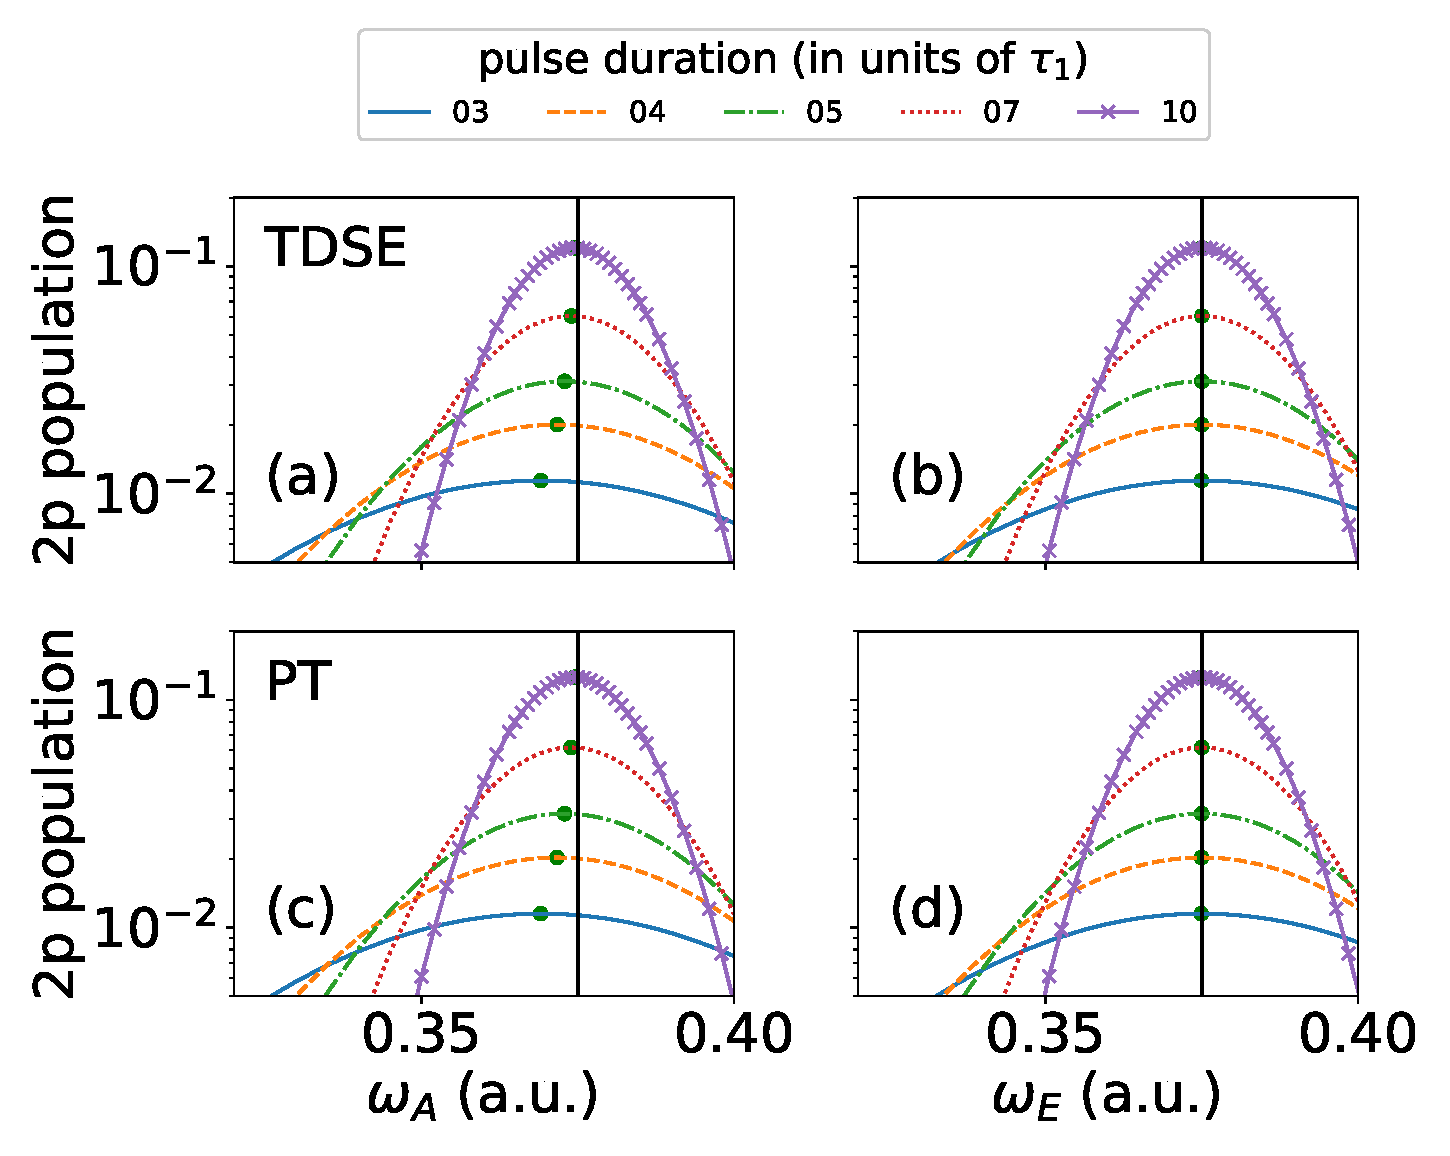
\includegraphics[width=\linewidth]{figs/2p_population_comb.eps}
\caption{(Color online)
Population in $2p$ state following one-photon excitation of hydrogen atom with a laser pulse as a function of $\omega_A$ (left) and $\omega_E$ (right) for different pulse lengths at peak intensity $10^{12}$ W/cm$^2$. Each line represents results obtained for a fixed pulse duration in terms of $\tau_1=405$ as. The results from time-dependent Schr\"odinger equation (TDSE) calculations (a,b) and predictions within first-order perturbation theory (PT) (c,d) are in excellent agreement. The vertical line marks the energy difference between $2p$ and initial $1s$ state. The green dots indicate the maximum excited state population for each pulse duration. 
}
  \label{fig:h-excited_2p}
\end{figure}

We have also obtained the population in the $2p$ state due to single photon excitation by direct numerical solution of the TDSE. These numerical results are presented together with those obtained within first order perturbation theory, Eq.~(\ref{perturbation}), in Fig.~\ref{fig:h-excited_2p} as function of $\omega_A$ (left column) and $\omega_E$ (right column) for various pulse lengths. The pulse length $\tau$ is measured in multiples of the period associated with the resonant frequency
\begin{equation}
\tau_{n_p} = \frac{2\pi}{\omega_{res}} = \frac{2\pi n_p}{|E_\text{final}-E_\text{initial}|},
\end{equation}
such that $\tau_1\approx 405$ attoseconds, $\tau_2 \approx 811$ attoseconds and so on for the $1s \rightarrow 2p$ transition. For long pulses the peak in the population (marked by a green dot) occurs at the expected frequency $\omega_\text{res}$ (marked by vertical line) for a resonant transition in all distributions. When the pulse length is decreased, the peak in the distributions as a function of $\omega_E$ (right column) remains at $\omega_\text{res}$. In contrast, the peak shifts significantly towards lower frequencies in the distributions as a function of $\omega_A$ (left column) due to the frequency shift. We note that the results of our numerical calculations (upper row) are in excellent agreement with those obtained using first-order perturbation theory (lower row) and indeed both reveal the same dependence on the central frequencies $\omega_A$ and $\omega_E$. Thus, the differences in the distributions as functions of $\omega_A$ and $\omega_E$ are not a numerical artifact but are due to the frequency shift. Furthermore, the observed shift agrees with our estimate obtained in the previous section. Thus, we can conclude that the central frequency of the electric field is the physically relevant quantity for interpreting laser induced excitation processes.


\begin{figure}[t]
\centering
       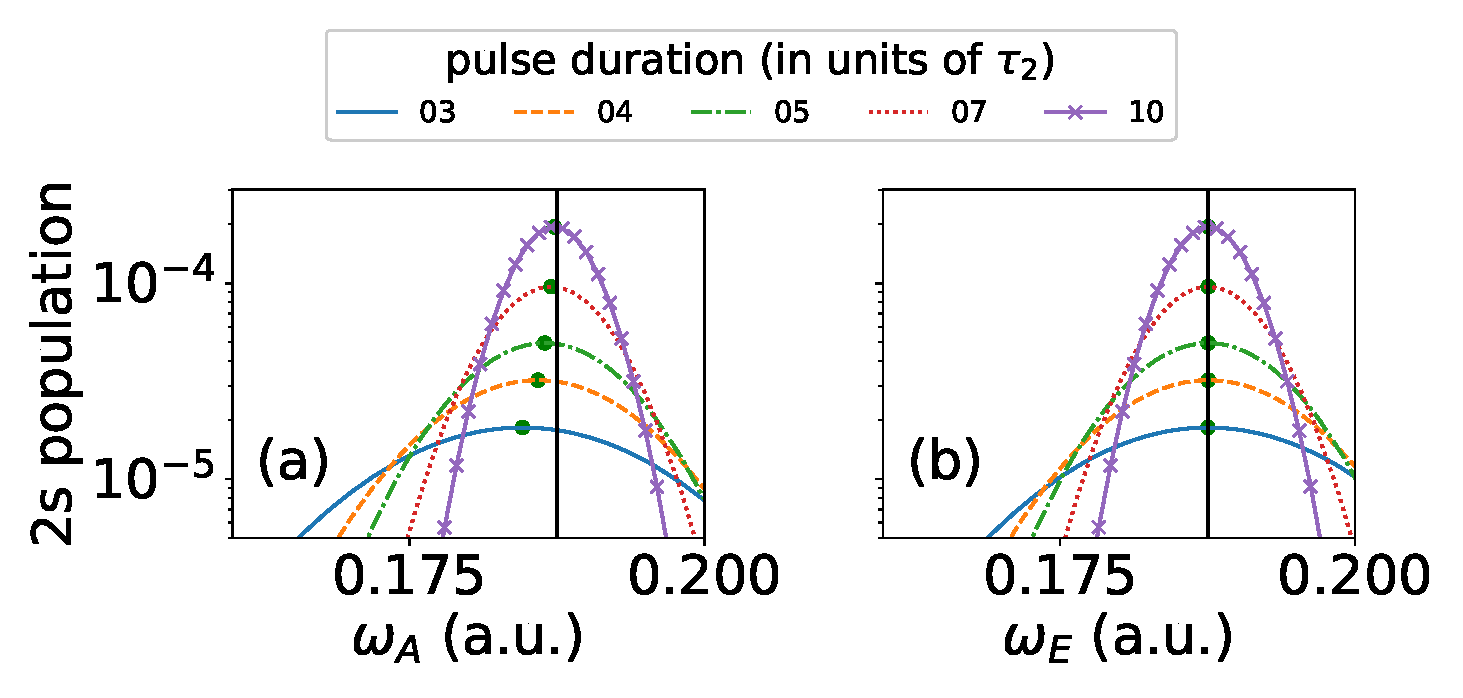
\includegraphics[width=\linewidth]{figs/Frequency_shift/2s_population_comb.eps}
\caption{(Color online)
Numerical results for population in $2s$ state following 2-photon excitation with $\tau_2=811$ as. The vertical line marks half of the energy gap between $1s$ and $2s$ representing the resonance condition for the two photon process. Other parameters are the same as in Fig. \ref{fig:h-excited_2p}.
}
  \label{fig:h-excited_2s}
\end{figure}

These conclusions are further supported by our numerical results for two-photon excitation from the $1s$ to the $2s$ state in Fig.~\ref{fig:h-excited_2s}. Whereas the peak of the population as a function of $\omega_E$ (panel b) occurs at $\omega_\text{res}$, independent of the pulse duration, the peak of the population as a function of  $\omega_A$ once again shifts to lower frequencies in Fig.~\ref{fig:h-excited_2s}(a). We note that, if the population as function of $\omega_A$ in Figs.~\ref{fig:h-excited_2p} and \ref{fig:h-excited_2s} were used to determine the energy difference $|E_\text{final} - E_\text{initial}|$, the error caused by the frequency shift would be twice as much in the two-photon case as in the one-photon case, accounting for the difference in $\tau_{n_p}$. This indicates that multiphoton processes may be affected by the frequency shift even more than few-photon processes. To further illustrate this point, we examine high harmonic generation in subsection~\ref{sec:HHG}.


Finally, we consider a highly nonlinear laser induced process. High harmonic generation (HHG) in atoms can be described as absorption of an odd number of photons leading to the excitation of a electron, followed by the emission of a single photon as the electron recombines into the ground state. Based on the results above, we expect that in this nonlinear process the frequency shift $\Delta\omega$ between $\omega_A$ and $\omega_E$ will lead to a shift of the energy of the $n_p$th harmonic by $n_p\Delta\omega$. In our calculations the HHG spectrum has been obtained by a Fourier transformation of the time dependent dipole acceleration along the laser polarization direction. A Hanning filter was used to return the dipole acceleration to zero at the beginning and end of the simulation. 

\begin{figure*}[t]
\centering
    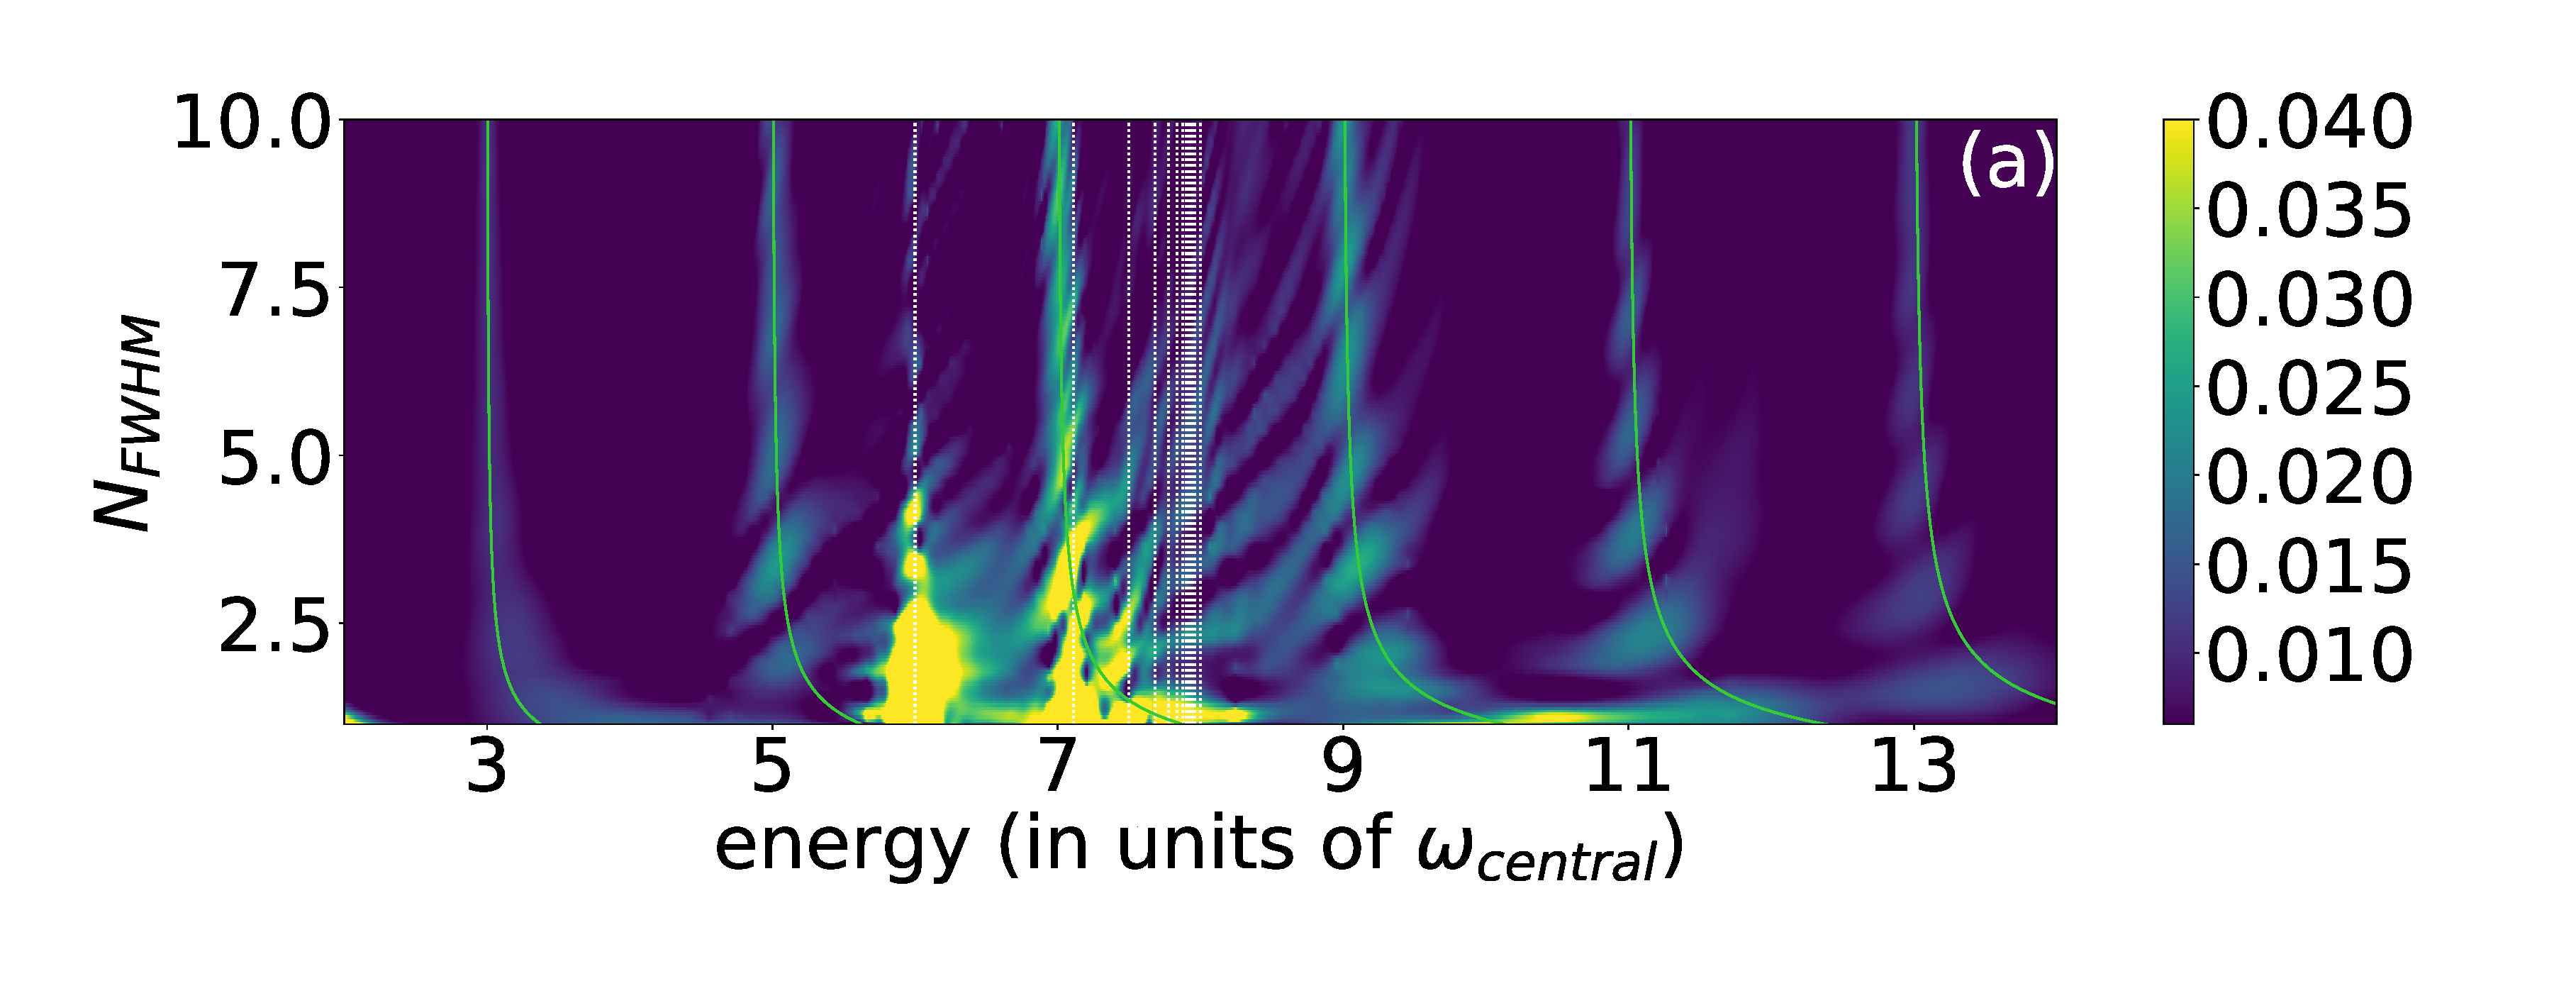
\includegraphics[width=\linewidth]{figs/Frequency_shift/HHG_w_A.eps}       
    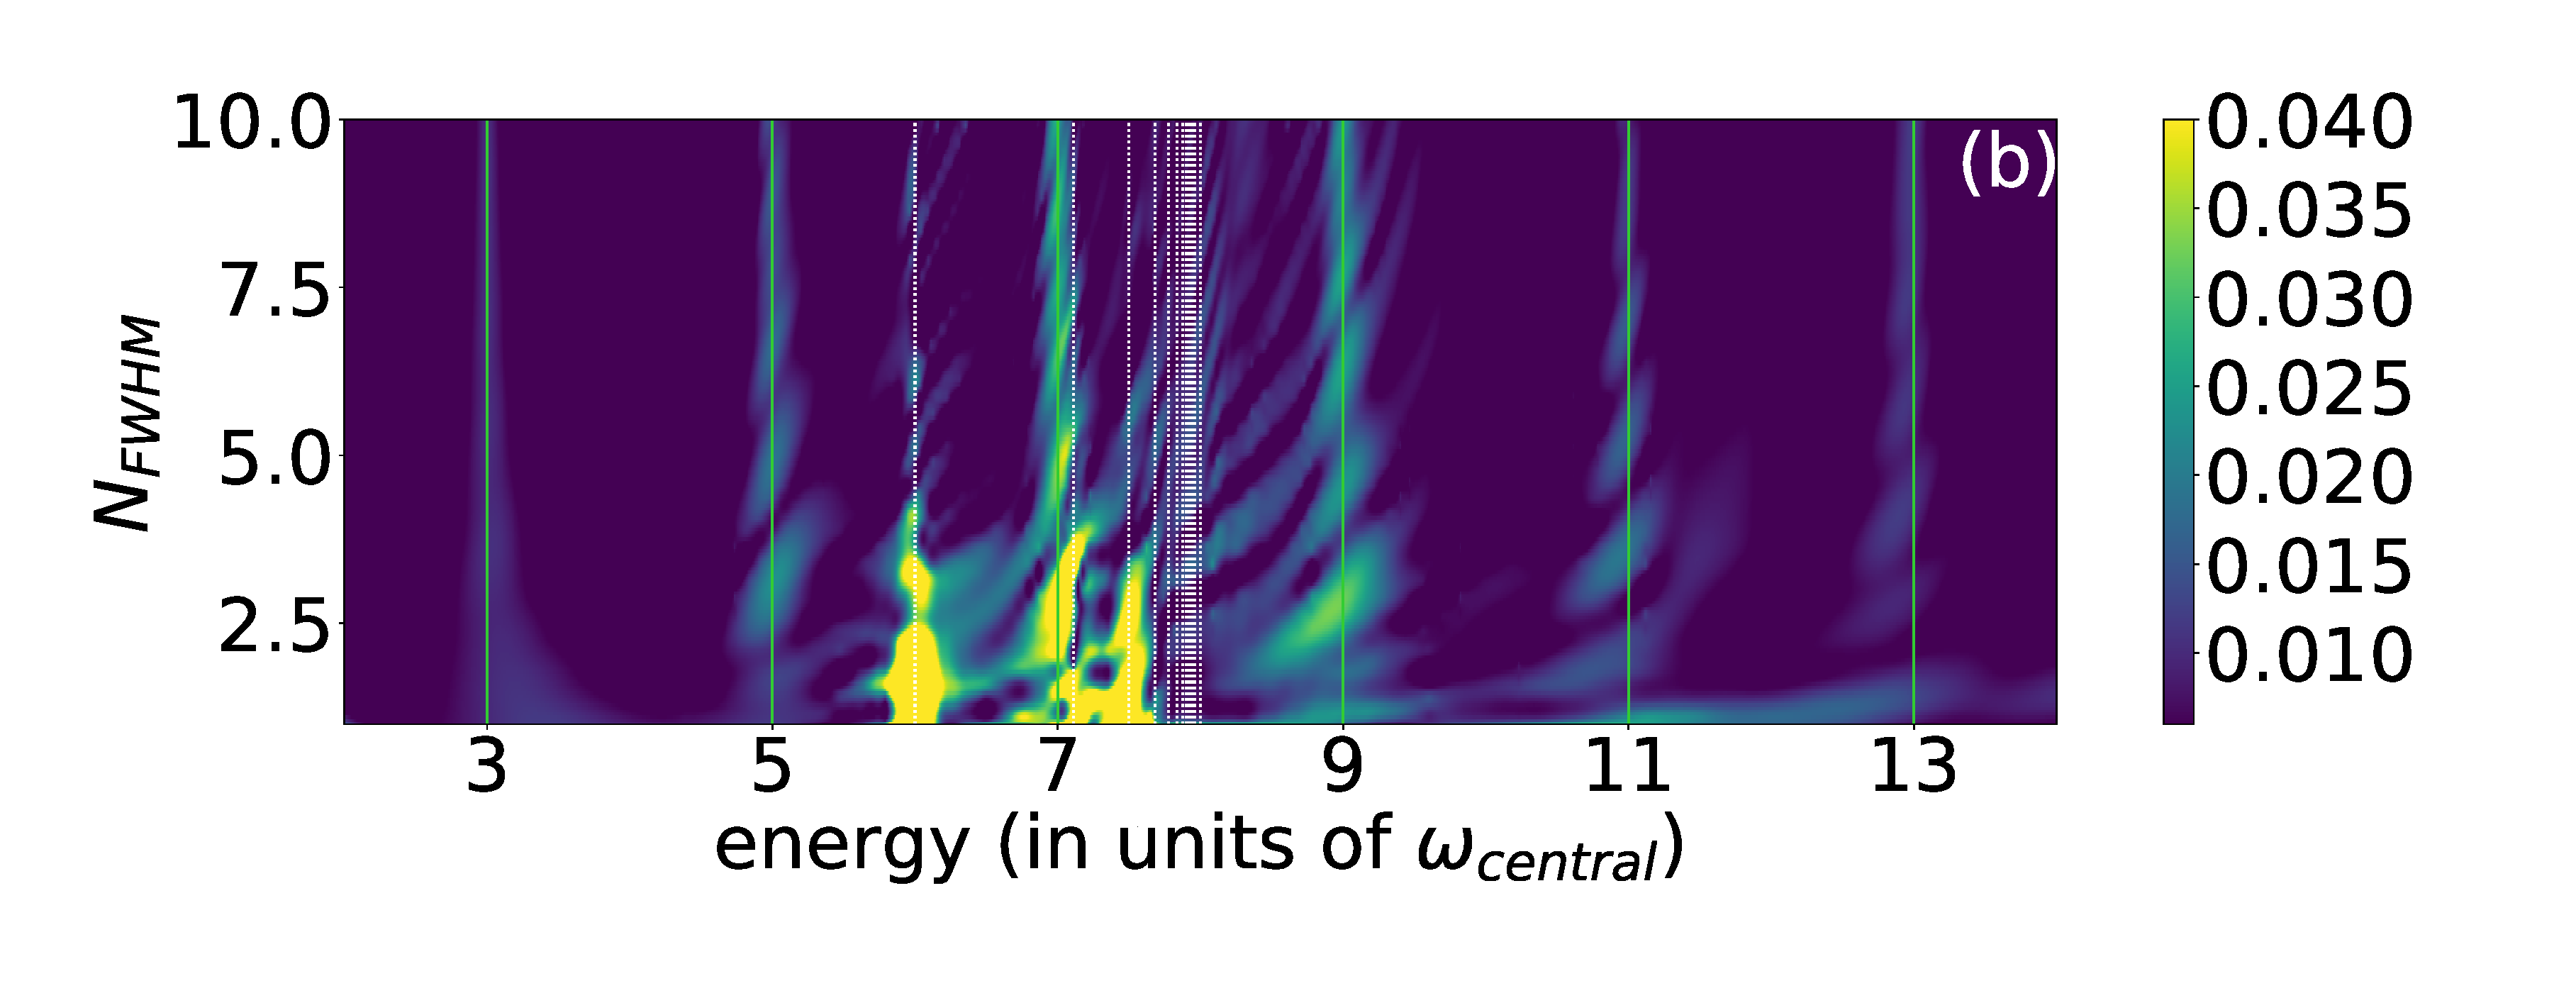
\includegraphics[width=\linewidth]{figs/Frequency_shift/HHG_w_E.eps}
\caption{(Color online)
HHG spectrum at driver wavelength 730 nm ($\omega_\text{central}$ = 0.0625 a.u.) vs.\ number of cycles $N_\text{FWHM}$. In the upper plot the central frequency $\omega_A = \omega_\text{central}$ while in the lower panel $\omega_E = \omega_\text{central}$. The vertical white dashed lines mark field-free transition energies between excited states and the ground state, while the green solid lines mark the harmonic energies $n_p\omega_E$ with respect to the central frequency of the electric field.
}
  \label{fig:HHG}
\end{figure*}

Fig.~\ref{fig:HHG} shows the various harmonics in a HHG spectrum as a function of the number of cycles in the driving laser pulse at a peak intensity of $1\times 10^{14}$ W/cm$^2$ and central frequencies $\omega_A=0.0625$ a.u.\ \ (upper panel) and $\omega_E=0.0625$ a.u.\ \ (lower panel), corresponding to a wavelength of 730 nm. The spectrum consists of odd harmonics and additional emission lines due to the population of excited states during the interaction with the laser pulse. While we will focus on the generation of harmonics, we note that the emission lines occur at photon energies between the 5th and 9th harmonics. The corresponding field-free energy differences between the excited states and the ground state in our numerical model of the hydrogen atom are marked, as reference, by white vertical dashed lines.

In the spectrum as function of multiples of $\omega_A$ (panel a) one can see that the centers of the harmonics do shift to energies larger than $n_p\omega_A$, as the pulse duration decreases. In fact, the energies of the harmonics follow the analytical predictions for $n_p\omega_E$ (green solid lines). As expected, the shift is as larger as larger the harmonic number. In contrast, in the HHG spectrum obtained as multiples of $\omega_E$ (panel b) the centers of the harmonics remain at the same energy, i.e.~$n_p\omega_E$ (green solid lines), as the pulse duration decreases. This confirms the importance of the shift between the central frequencies of the vector potential and the electric field in nonlinear processes driven by ultrashort pulses. Furthermore, the HHG results confirm that the central frequency of the electric field $\omega_E$ is the physical relevant quantity for the interpretation of light induced processes. Consequently, if in a numerical simulation or theoretical analysis the vector potential is set via Eq.~(\ref{eq:vectorpotential}) it is necessary to consider the frequency shift between $\omega_A$ and $\omega_E$ to avoid a misinterpretation of the results. Our analytical estimates of the frequency shift in Eq.~(\ref{eq:fshiftapprox}) and Eq.~(\ref{eq:alternative}) provide formulas to obtain $\omega_A$ from the physically relevant $\omega_E$.


We have shown that the definition of the electric field of a laser pulse via the derivative of the vector potential, which guarantees that both quantities vanish at the beginning and end of the pulse, implies that the central frequencies of the spectral distributions of the vector potential and electric field do not coincide. 

In our analysis we have derived an analytical estimate of the frequency shift, which shows that the shift mainly depends on the number of cycles in the pulse and becomes most relevant for few-cycle pulses. Utilizing results of numerical simulations and first-order perturbation theory we have analyzed how the frequency shift affects excitation, ionization and high harmonic generation induced by short laser pulses. The effect is found to be most noticeable in nonlinear strong-field processes since the frequency shift scales with the number of photons involved. Both, numerical results and predictions based on first-order perturbation theory agree well with each other and confirm that the central frequency of the electric field is the physically relevant quantity for the interpretation of the light induced processes. Thus, the shift should be taken into account when setting the central frequency of the vector potential in numerical simulations to avoid potential misinterpretation of the theoretical results, specifically when compared to experimental data. Eq.~(\ref{eq:fshiftapprox}) and Eq.~(\ref{eq:alternative}) provide formulas to obtain $\omega_A$ from the physically relevant $\omega_E$.

% section laser_pulses (end)

